\chapter{古典概率模型}
\label{chap:classical-probability}

掷两枚骰子，点数和是$7$的可能性有多大？盒子里有$3$个黑球、$2$个白球，不放回地摸出两个，两个都是黑球的可能性又有多大？这两个问题的结果事先都不确定，但我们都愿意给出一个确定的数。只要相信骰子的六个面、盒中的五个球“机会均等”，概率就变成了计数：数一数有利的结果，再除以全部结果。

计数看起来简单，出错却很容易。两枚骰子的点数和只有$11$种，它们并不同样可能；摸球时记不记录先后次序，结果的总数会差一倍；分子按一种口径数、分母按另一种口径数，得到的数就没有意义。本章的第一个任务，是学会把一个概率问题准确地翻译成计数问题：先写清楚一次试验可能产生哪些结果，再判断哪些结果可以看作等可能，最后按同一口径数出分子和分母。

第二个任务是处理信息。如果已经知道第一个球是黑球，第二个球是黑球的可能性就从$3/5$变成了$2/4$；如果知道一件产品在检测中报警，它是次品的可能性也会随之改变。处理办法是把样本范围缩小到已知发生的那些结果，再在其中重新计算比例。由这一步可以得到逐步相乘的计算规则，也可以按来源分组，再从观测结果反推它来自哪一组。

最后讨论概率在什么时候可以直接相乘。放回摸球时第一次的结果不影响第二次，不放回时则不然；“互不影响”需要一个准确的数量定义。我们会看到，重复试验中这种互不影响来自对整个试验的等可能假设，而不是来自“看起来无关”。本章结尾说明计数比的适用边界：结果不等可能、结果有无穷多个或取连续位置时，它都不再适用，需要后面几章用别的方式分配概率。

\section{随机试验}
\label{sec:cprob-experiments}

掷一枚骰子之前，我们不知道会出现几点，却清楚地知道只可能是$1,2,\ldots,6$中的一个。摸球、抽牌、抽检产品都有同样的结构：结果事先不确定，但全部可能结果事先可以列出。要谈“可能性有多大”，先要说清“什么的可能性”，也就是把可能结果和我们关心的问题写成数学对象。

\paragraph{样本空间与样本点}
在相同条件下可以重复进行、每次恰好产生一个结果、而全部可能结果事先已知的试验，称为\term{随机试验}（random experiment）。掷骰子、从盒中摸球、从一副牌中抽牌都是随机试验。一次试验究竟产生哪个结果事先不知道，概率要描述的正是这种不确定性。

\begin{definition}[样本空间与事件]
\label{def:cprob-sample-space}
随机试验全部可能结果组成的集合称为\term{样本空间}（sample space），记为$\Omega$，其元素$\omega$称为\term{样本点}（sample point）。样本空间的子集称为\term{事件}（event）。本章只讨论有限的样本空间，此时$\Omega$的每个子集都是事件。
\end{definition}

掷一枚骰子时，$\Omega=\{1,2,3,4,5,6\}$，“出现偶数点”是事件$\{2,4,6\}$，“点数大于$4$”是事件$\{5,6\}$。事件只是满足某个条件的那些结果放在一起，条件可以用文字说，也可以把元素列出来，两种写法指同一个集合。

整个样本空间$\Omega$也是事件，它包含全部结果，每次试验都发生，称为\term{必然事件}（certain event）。空集$\varnothing$不含任何结果，从不发生，称为\term{不可能事件}（impossible event）。只含一个样本点的事件$\{\omega\}$称为\term{基本事件}（elementary event）。

\paragraph{实际结果与事件}
试验做完以后，实际出现的是一个确定的样本点$\omega$。事件则是事先提出的问题，例如“会不会出现偶数点”。若实际结果$\omega\in A$，就说事件$A$在这次试验中\emph{发生}了，否则说它没有发生。

两者的区别在于数量。一次试验只产生一个结果，却可以同时让许多事件发生。设骰子掷出了$4$，那么$\{2,4,6\}$、$\{4,5,6\}$、$\{4\}$和$\Omega$都发生了，$\{1,3,5\}$和$\{5,6\}$没有发生。概率是对事件提出的，它在试验之前就有意义；试验之后，每个事件只剩下“发生”或“没发生”两种状态。

\paragraph{事件的运算}
事件既然是集合，集合运算就对应事件之间的逻辑组合，集合的记号可参考\BookChapterRef{chap:sets-relations-maps}{卷一第1章“集合、关系与映射”}。设$A,B$是事件：
\begin{itemize}
 \item 并$A\cup B$表示“$A$与$B$至少有一个发生”；
 \item 交$A\cap B$表示“$A$与$B$同时发生”；
 \item 补$A^{\mathrm{c}}=\Omega\setminus A$表示“$A$不发生”；
 \item 差$A\setminus B=A\cap B^{\mathrm{c}}$表示“$A$发生而$B$不发生”。
\end{itemize}

把$\Omega$画成矩形，把事件画成其中的区域，这些运算就是区域的合并、重叠和剩余，如图~\ref{fig:cprob-event-operations}所示。De Morgan律
\[
 (A\cup B)^{\mathrm{c}}=A^{\mathrm{c}}\cap B^{\mathrm{c}},\qquad
 (A\cap B)^{\mathrm{c}}=A^{\mathrm{c}}\cup B^{\mathrm{c}}
\]
读作：“至少一个发生”的反面是“两个都不发生”，“两个同时发生”的反面是“至少一个不发生”。后面计算“至少一个”时，常借这条规律转到它的反面。

\begin{BookInlineFigure}
  \centering
  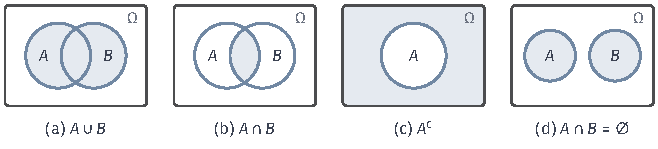
\includegraphics[width=112mm]{figures/07-probability/01-elementary-probability/tikz/cprob-event-operations/figure.pdf}
  \caption{事件的运算。矩形是样本空间$\Omega$，圆是事件，浅蓝区域是运算得到的事件。(a)并；(b)交；(c)补；(d)两个没有公共结果的事件。}
  \label{fig:cprob-event-operations}
\end{BookInlineFigure}

若$A\cap B=\varnothing$，即$A$与$B$没有公共的结果，就称它们\term{互斥}（mutually exclusive），如图~\ref{fig:cprob-event-operations}(d)。互斥的事件不能在同一次试验中同时发生。掷骰时“出现偶数点”与“出现$1$点”互斥；“出现偶数点”与“点数大于$4$”不互斥，结果$6$同时属于二者。

\paragraph{记录方式决定样本空间}
同一个物理过程可以用不同的方式记录，记录方式不同，样本空间就不同。下面用一个摸球问题说明这一点，本章后面会反复回到它：盒中有$5$个球，编号$1,2,3$的是黑球，编号$4,5$的是白球，搅匀后不放回地依次摸出两个。

第一种记录是按先后写下两个球的编号，结果是有序对$(a,b)$，$a\neq b$。第一个球有$5$种可能，第二个球有$4$种，样本空间有$5\times4=20$个点。第二种记录只写下摸到了哪两个球，不管先后，结果是二元子集$\{a,b\}$，共$\binom52=10$个。第三种只记颜色，结果是“黑黑”“黑白”“白黑”“白白”四种。

图~\ref{fig:cprob-urn-records}把三种样本空间并排画出。事件“两个都是黑球”在三种记录下分别是$6$个有序对、$3$个子集和$1$个颜色记录。三种记录描述的是同一件事，但样本点的个数不同，样本点所代表的情形也不同：一个颜色记录“黑黑”合并了$6$个有序对。

\begin{BookInlineFigure}
  \centering
  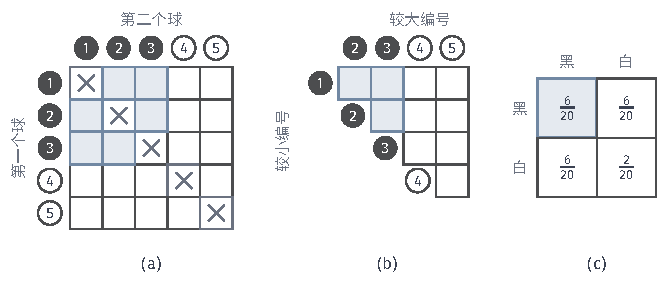
\includegraphics[width=112mm]{figures/07-probability/01-elementary-probability/tikz/cprob-urn-records/figure.pdf}
  \caption{不放回摸两个球的三种记录。实心圆是黑球$1,2,3$，空心圆是白球$4,5$；浅蓝格子是事件“两个都是黑球”。(a)有序对：行是第一个球，列是第二个球，对角线上的格子不可能出现，共$20$个结果。(b)无序对：只保留编号较小者在行、较大者在列的$10$个格子。(c)颜色记录：行、列分别是第一、第二个球的颜色，格中数字是(a)中相应格子数占$20$的比例，四个结果并不同样可能。}
  \label{fig:cprob-urn-records}
\end{BookInlineFigure}

选择样本空间要满足两个要求。第一，它必须细到能表达所关心的事件。事件“第一个球是黑球”在有序记录中是$12$个有序对，在无序记录中却写不出来：子集$\{1,4\}$既可能是先摸到$1$，也可能是先摸到$4$。第二，它最好让每个样本点同样可能，这样概率才能靠计数得到。

颜色记录满足第一个要求，却不满足第二个：图~\ref{fig:cprob-urn-records}(c)中“白白”只对应$2$个有序对，“黑黑”对应$6$个。下一节把“同样可能”写成模型假设，并说明为什么有序记录满足它而颜色记录不满足。

若改为放回摸球，即摸出一个球记下编号后放回盒中，再摸第二个，那么第二个球可以与第一个相同，有序记录的样本空间就是全部$5\times5=25$个有序对，图~\ref{fig:cprob-urn-records}(a)中对角线上的$5$个格子也成为可能结果。放回与否改变的是样本空间本身，而不只是某个事件。

\section{等可能模型}
\label{sec:cprob-equally-likely}

一枚做工均匀的骰子，六个面在形状和重量上没有区别，我们找不到任何理由认为某一面更容易朝上。既然如此，就让六个面分得同样多的可能性，各占$1/6$。“出现偶数点”包含三个面，它的可能性就是$3/6$。把这个想法推广到一般的有限样本空间，就得到用计数定义的概率。

\paragraph{计数比}
可以把概率想成一份总量为$1$的质量，要分配到样本空间的各个点上。等可能就是平均分配：$\Omega$有$\lvert\Omega\rvert$个点，每个点分到$1/\lvert\Omega\rvert$。一个事件的概率，就是落在这个事件区域里的质量总和。点的质量相同，总和就等于点数乘以每点的质量。

\begin{definition}[古典概率]
\label{def:cprob-classical}
设样本空间$\Omega$有限且非空，并假设每个样本点同样可能出现。对每个事件$A\subseteq\Omega$，令
\begin{equation}
 \mathbb{P}(A)=\frac{\lvert A\rvert}{\lvert\Omega\rvert},
 \label{eq:cprob-classical}
\end{equation}
其中$\lvert A\rvert$是$A$的元素个数。称$\mathbb{P}(A)$为事件$A$的概率，称$(\Omega,\mathbb{P})$为\term{古典概率模型}（classical probability model）。
\end{definition}

式~\eqref{eq:cprob-classical}把概率问题完全化成了计数问题：分子数事件里的结果，分母数全部结果，两者都在同一个样本空间里数。每个基本事件的概率都是$1/\lvert\Omega\rvert$，这正是“等可能”的数学表述。

\paragraph{三条基本性质}
这个定义给出的数满足哪些规律？我们希望概率像“占比”一样运算：不会是负数，全体的占比是$1$，两块不重叠的部分合起来，占比相加。下面验证计数比确实具有这三条性质；后面的一切运算规则都从它们推出。

\begin{theorem}[古典概率的基本性质]
\label{thm:cprob-axioms}
在古典概率模型中，对任意事件$A,B$：
\begin{enumerate}
 \item 非负性：
 \begin{equation}
  \mathbb{P}(A)\geq0;
  \label{eq:cprob-nonneg}
 \end{equation}
 \item 归一性：
 \begin{equation}
  \mathbb{P}(\Omega)=1;
  \label{eq:cprob-normalized}
 \end{equation}
 \item 互斥可加性：若$A\cap B=\varnothing$，则
 \begin{equation}
  \mathbb{P}(A\cup B)=\mathbb{P}(A)+\mathbb{P}(B).
  \label{eq:cprob-additive}
 \end{equation}
\end{enumerate}
\end{theorem}

\begin{proof}
元素个数非负，分母$\lvert\Omega\rvert$为正，所以$\mathbb{P}(A)\geq0$。取$A=\Omega$，分子分母相同，比值为$1$。

若$A\cap B=\varnothing$，并集$A\cup B$中的每个元素恰好属于$A$与$B$中的一个，按计数的加法规则
\[
 \lvert A\cup B\rvert=\lvert A\rvert+\lvert B\rvert.
\]
两边同除以$\lvert\Omega\rvert$，就得到式~\eqref{eq:cprob-additive}。
\end{proof}

互斥可加性对有限个两两互斥的事件同样成立。设$A_1,\ldots,A_m$两两互斥，对$m$归纳：$A_1\cup\cdots\cup A_{m-1}$与$A_m$互斥，用一次式~\eqref{eq:cprob-additive}，再用归纳假设，得到
\[
 \mathbb{P}(A_1\cup\cdots\cup A_m)=\mathbb{P}(A_1)+\cdots+\mathbb{P}(A_m).
\]
特别地，任何事件都是它所含基本事件的互斥并，所以$\mathbb{P}(A)$等于$A$中各点概率之和。这与开头“质量总和”的图景一致。

反过来，计数比也是唯一与等可能相容的分配。设某种分配满足三条基本性质，并且每个基本事件的概率都等于同一个数$c$。$\Omega$是它的$\lvert\Omega\rvert$个基本事件的互斥并，由有限可加性与归一性，
\[
 1=\mathbb{P}(\Omega)=\lvert\Omega\rvert\,c,
\]
所以$c=1/\lvert\Omega\rvert$；再对$A$的各点求和，就得到$\mathbb{P}(A)=\lvert A\rvert/\lvert\Omega\rvert$。因此定义~\ref{def:cprob-classical}并没有额外的选择：一旦接受等可能假设和三条性质，概率只能是计数比。

\paragraph{两枚骰子}
掷两枚骰子，把它们看成可区分的第一枚与第二枚，结果记为有序对$(i,j)$，$i,j\in\{1,\ldots,6\}$。样本空间有$36$个点。若每枚骰子都均匀，两次投掷互不干扰，我们就假设这$36$个有序对同样可能。

图~\ref{fig:cprob-dice-grid}把$36$个结果排成方格，格中写的是点数和$i+j$。点数和相同的格子排在同一条斜线上。事件“点数和为$7$”占$6$格，“点数和为$2$”只占$1$格，于是
\[
 \mathbb{P}(\text{点数和为}7)=\frac{6}{36}=\frac16,\qquad
 \mathbb{P}(\text{点数和为}2)=\frac{1}{36}.
\]

\begin{BookInlineFigure}
  \centering
  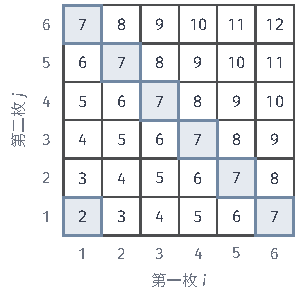
\includegraphics[width=51mm]{figures/07-probability/01-elementary-probability/tikz/cprob-dice-grid/figure.pdf}
  \caption{两枚骰子的$36$个等可能结果。横向是第一枚的点数$i$，纵向是第二枚的点数$j$，格中数字是点数和。浅蓝格子是事件“点数和为$7$”（$6$格）与“点数和为$2$”（$1$格）。}
  \label{fig:cprob-dice-grid}
\end{BookInlineFigure}

点数和从$2$到$12$共$11$种。如果以这$11$个值为样本点，并认为它们同样可能，每个值的概率就都是$1/11$。这与计数结果矛盾：和为$7$的出法有$6$种，和为$2$只有$(1,1)$一种。以点数和为样本点并没有错，错的是对它们使用了等可能假设。

\paragraph{等可能是模型假设}
上面的矛盾说明，式~\eqref{eq:cprob-classical}的前提“每个样本点同样可能”不是从样本空间的写法推出来的，而是对试验所作的假设。它的依据是试验的物理对称性：骰子各面均匀，牌洗得充分，摸球前搅匀且每个球被摸到的机会相同。样本点的名称看起来对称，并不构成这样的依据。

历史上一个有名的错误是这样的：抛两枚硬币，结果分为“两正”“两反”“一正一反”三种，于是认为每种的概率都是$1/3$。按硬币区分先后，等可能的结果是“正正”“正反”“反正”“反反”四种，“一正一反”占了其中两种，所以
\[
 \mathbb{P}(\text{两正})=\frac14,\qquad
 \mathbb{P}(\text{一正一反})=\frac12.
\]
三种结果的名称同样简单，但它们合并的基本结果个数不同，不能平分概率。

哪个模型对，可以用重复试验来检验。把同一试验重复许多次，事件发生的次数除以试验次数称为事件的\term{相对频率}（relative frequency）。图~\ref{fig:cprob-coin-frequency}模拟了$2000$轮抛两枚硬币：随着轮数增加，“两正”的相对频率稳定在$1/4$附近，“一正一反”稳定在$1/2$附近，都远离$1/3$。

\begin{BookInlineFigure}
  \centering
  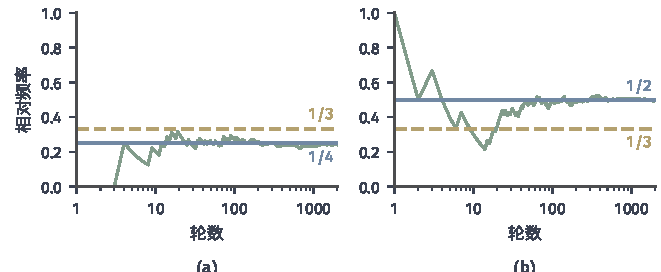
\includegraphics[width=112mm]{figures/07-probability/01-elementary-probability/matplotlib/cprob-coin-frequency/figure.pdf}
  \caption{抛两枚均匀硬币$2000$轮的模拟（随机数种子$3$），横轴为对数坐标。绿线是前若干轮中事件的相对频率，蓝线是四个有序结果等可能时的概率，黄色虚线是错误地认为三种结果等可能时的$1/3$。(a)两正；(b)一正一反。$2000$轮后两个频率分别是$0.2415$和$0.496$。}
  \label{fig:cprob-coin-frequency}
\end{BookInlineFigure}

图~\ref{fig:cprob-dice-sum-frequency}对两枚骰子做了同样的检验。$3600$次模拟中，各点数和的相对频率紧贴计数比$k/36$，其中$k$是该点数和所占的格子数；它们与$1/11$的水平线则明显不符。

\begin{BookInlineFigure}
  \centering
  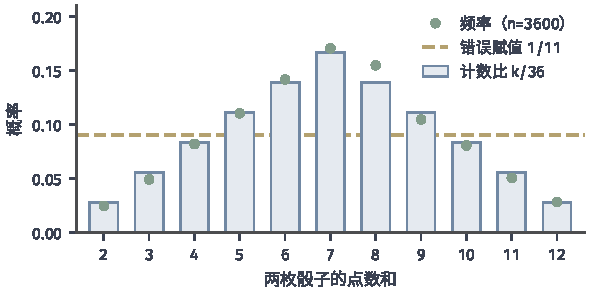
\includegraphics[width=100mm]{figures/07-probability/01-elementary-probability/matplotlib/cprob-dice-sum-frequency/figure.pdf}
  \caption{两枚骰子点数和的概率与频率。浅蓝柱是$36$个有序结果等可能时的概率$k/36$，绿点是$3600$次模拟中的相对频率（随机数种子$7$），黄色虚线是错误地把$11$个点数和看作等可能时的$1/11$。}
  \label{fig:cprob-dice-sum-frequency}
\end{BookInlineFigure}

\paragraph{古典概率与频率}
古典概率和相对频率回答的是不同的问题。古典概率由模型算出，是一个确定的数，不依赖任何实际的投掷；相对频率由观察得到，每做一批试验结果都不同，图~\ref{fig:cprob-coin-frequency}中前几十轮的波动很大。前者是对试验的假设所推出的结论，后者是对试验本身的记录。

两者的联系是：如果模型的等可能假设与试验相符，相对频率在大量重复中会靠近模型给出的概率；如果明显偏离，就说明假设与试验不符，例如一枚灌铅的骰子会让某一面的频率持续偏高。“频率靠近概率”在什么意义下成立，需要先有独立重复试验和随机变量的语言，这一结论在第~\ref{chap:laws-of-large-numbers}章证明。本章只把频率当作检验模型的经验依据，不用它来定义概率。

\paragraph{再看摸球问题}
回到第~\ref{sec:cprob-experiments}节的摸球问题。搅匀后摸球，每个球被第一个摸到的机会相同；摸走一个以后，剩下的四个球被第二个摸到的机会也相同。所以$20$个有序对同样可能，有序记录满足等可能假设。

在有序记录中，“两个都是黑球”有$3\times2=6$个结果，“第一个黑、第二个白”有$3\times2=6$个，“第一个白、第二个黑”有$2\times3=6$个，“两个都是白球”有$2\times1=2$个。于是四个颜色记录的概率分别是
\[
 \frac{6}{20},\quad \frac{6}{20},\quad \frac{6}{20},\quad \frac{2}{20}.
\]
这就是图~\ref{fig:cprob-urn-records}(c)中的数。颜色记录可以作为样本空间，但它的四个点不等可能，不能用计数比；它们的概率要从有序记录算出。第~\ref{sec:cprob-scope}节会专门讨论这种合并带来的问题。

\section{事件概率的计算}
\label{sec:cprob-computing}

有了式~\eqref{eq:cprob-classical}，计算概率就是数两个集合。真正的困难在于数对：样本空间要选得等可能，事件要在同一个样本空间里数，补、并、交这些组合事件要用合适的方式拆开。本节先整理抽样问题中常用的计数公式，再分别处理补事件、并事件和交事件。

\paragraph{四种抽样方式}
从$n$个可区分的对象中取$k$次，按“是否放回”和“是否记录次序”可以分成四种情形。各自的结果个数在\BookChapterRef{chap:counting}{卷一第2章“计数”}中已经得到，记$P(n,k)=n(n-1)\cdots(n-k+1)$为排列数，$\binom nk$为组合数。表~\ref{tab:cprob-sampling}把它们放在一起，并标出每种记录下的结果是否同样可能。

\begin{BookInlineTable}
  \centering
  \caption{从$n$个对象中取$k$次的四种记录方式}
  \label{tab:cprob-sampling}
  \begin{tabular}{llll}
    \toprule
    记录方式 & 结果的形式 & 结果个数 & 是否等可能 \\
    \midrule
    不放回、有序 & 无重复的$k$元有序组 & $P(n,k)$ & 是 \\
    不放回、无序 & $k$元子集 & $\binom nk$ & 是 \\
    放回、有序 & 可重复的$k$元有序组 & $n^{k}$ & 是 \\
    放回、无序 & 可重复的$k$元组合 & $\binom{n+k-1}{k}$ & 否 \\
    \bottomrule
  \end{tabular}
\end{BookInlineTable}

前三种的等可能性来自同一个物理假设：每次取样时，剩下的各对象被取到的机会相同。有序记录直接继承这一假设。不放回的无序记录中，每个$k$元子集恰好由$k!$个有序组忘去次序得到，各子集合并的有序组个数相同，所以仍等可能。放回的无序记录则不然：取两次时，组合$\{1,1\}$只来自有序组$(1,1)$，组合$\{1,2\}$却来自$(1,2)$和$(2,1)$两个。这一行不能直接用于计数比，第~\ref{sec:cprob-scope}节再回到它。

\paragraph{分子与分母同一口径}
在摸球问题中计算“两个都是黑球”的概率。用有序记录，分母是$P(5,2)=20$，分子是从$3$个黑球中有序地取$2$个，$P(3,2)=6$；用无序记录，分母是$\binom52=10$，分子是$\binom32=3$。两种算法给出
\[
 \frac{P(3,2)}{P(5,2)}=\frac{6}{20}=\frac{3}{10},\qquad
 \frac{\binom32}{\binom52}=\frac{3}{10}.
\]
结果一致。若分子用无序的$3$、分母用有序的$20$，就得到$3/20$，这个数不是任何事件的概率。

两种口径给出同一结果并非巧合。“两个都是黑球”只关心摸到了哪些球，不关心先后。对这样的事件，每个满足条件的子集恰好对应$k!$个满足条件的有序组，分子和分母同乘以$k!$，比值不变。这个论证也说明了口径一致的含义：分子和分母必须是同一个样本空间中的计数。

事件“恰好一个黑球”同样只与内容有关。无序记录中它有$3\times2=6$个子集，有序记录中有$3\times2\times2=12$个有序对，概率都是$3/5$。事件“第一个是黑球”则与次序有关，只能在有序记录中数：第一个位置有$3$种，第二个位置从剩下$4$个中任取，共$12$个，概率也是$3/5$。

\paragraph{一副牌中的组合计数}
从一副$52$张的扑克牌中随机抽$3$张，不放回。每个$3$张的子集同样可能。事件“$3$张都是红桃”要求$3$张全部取自$13$张红桃，所以
\[
 \mathbb{P}(\text{三张都是红桃})=\frac{\binom{13}{3}}{\binom{52}{3}}
 =\frac{286}{22100}=\frac{11}{850}\approx0.0129.
\]
第~\ref{sec:cprob-conditional}节会用逐张抽取的方式重新得到这个数。

事件较复杂时，常把满足条件的结果拆成几步来构造，再用乘法规则计数。这时要检查两件事：每一步的选择合起来恰好得到事件中的一个结果，事件中的每个结果也只由一种选择方式得到。以抽$5$张牌“恰好一对”为例，它要求有两张点数相同，其余三张的点数互不相同，也都不同于这一对。

按下面的步骤构造：先选成对的点数，有$13$种；再选这一对的两种花色，有$\binom42=6$种；再从其余$12$个点数中选出三个单张的点数，有$\binom{12}{3}=220$种；最后给三个单张各选一种花色，有$4^{3}=64$种。每手“恰好一对”的牌由唯一一组选择得到，所以
\[
 \mathbb{P}(\text{恰好一对})=\frac{13\times6\times220\times64}{\binom{52}{5}}
 =\frac{1098240}{2598960}\approx0.4226.
\]

一种常见的错误算法是：选好一对之后，从剩下的$48$张牌中任取$3$张，得到$13\times6\times\binom{48}{3}$。这样取出的三张可能又凑成一对，或与已选的一对同点数，于是两对、三条等牌型也被算了进去，而且一手两对的牌按“哪一对先选”会被数两次。另一种错误是把三个单张的点数按$12\times11\times10$有序地选，每手牌被重复数了$3!$次。两种错误都破坏了“恰好一个结果对应一种选择”。

\paragraph{补事件}
“至少一个”“不全相同”这类事件往往由许多情形组成，直接数很麻烦，它的反面却只有一种或少数几种情形。下面的公式把概率转到补事件上。

\begin{theorem}[补事件与包含关系]
\label{thm:cprob-complement}
在古典概率模型中，对任意事件$A$，
\begin{equation}
 \mathbb{P}(A^{\mathrm{c}})=1-\mathbb{P}(A).
 \label{eq:cprob-complement}
\end{equation}
若$A\subseteq B$，则
\begin{equation}
 \mathbb{P}(B\setminus A)=\mathbb{P}(B)-\mathbb{P}(A),\qquad
 \mathbb{P}(A)\leq\mathbb{P}(B)\leq1.
 \label{eq:cprob-monotone}
\end{equation}
特别地，$\mathbb{P}(\varnothing)=0$。
\end{theorem}

\begin{proof}
若$A\subseteq B$，则$B$是互斥的$A$与$B\setminus A$之并。由互斥可加性~\eqref{eq:cprob-additive}，
\[
 \mathbb{P}(B)=\mathbb{P}(A)+\mathbb{P}(B\setminus A).
\]
移项得到式~\eqref{eq:cprob-monotone}的等式；由非负性~\eqref{eq:cprob-nonneg}，$\mathbb{P}(B\setminus A)\geq0$，所以$\mathbb{P}(A)\leq\mathbb{P}(B)$。取$B=\Omega$，用归一性~\eqref{eq:cprob-normalized}，就得到式~\eqref{eq:cprob-complement}与$\mathbb{P}(B)\leq1$。再取$A=\Omega$，得到$\mathbb{P}(\varnothing)=1-1=0$。
\end{proof}

证明只用了三条基本性质，没有再回到计数。这一点后面很重要：凡是满足这三条性质的概率分配，补事件公式都成立。

\paragraph{生日问题}
一个班有$n$个人，至少两人同一天生日的概率是多少？作模型假设：一年按$365$天计，每人的生日在$365$天中等可能，各人之间互不影响。依次写下$n$个人的生日，结果是可重复的有序组，样本空间有$365^{n}$个等可能的点。

“至少两人同一天”包含两人相同、三人相同、两对分别相同等许多情形；它的补事件“$n$个生日两两不同”只有一种情形，正是不放回的有序取法，共$P(365,n)$个。由式~\eqref{eq:cprob-complement}，
\begin{equation}
 \mathbb{P}(\text{至少两人同一天生日})
 =1-\frac{P(365,n)}{365^{n}}
 =1-\prod_{i=0}^{n-1}\Bigl(1-\frac{i}{365}\Bigr).
 \label{eq:cprob-birthday}
\end{equation}

代入$n=23$，乘积约为$0.4927$，所求概率约为$0.5073$，已经超过一半；$n=50$时约为$0.970$。图~\ref{fig:cprob-birthday}画出了它随$n$的变化。这个结果常常出人意料，原因在于要比较的是人与人之间的配对，$23$个人之间有$\binom{23}{2}=253$对，每一对都可能撞上。

\begin{BookInlineFigure}
  \centering
  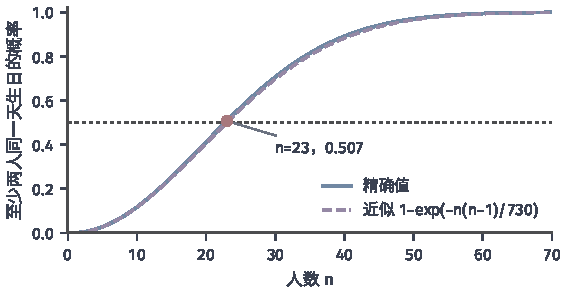
\includegraphics[width=96mm]{figures/07-probability/01-elementary-probability/matplotlib/cprob-birthday/figure.pdf}
  \caption{生日问题。蓝线是式~\eqref{eq:cprob-birthday}的精确值，紫色虚线是近似$1-\exp(-n(n-1)/730)$，黑色点线是$1/2$；红点标出$n=23$时的$0.507$。}
  \label{fig:cprob-birthday}
\end{BookInlineFigure}

配对的说法可以变成一个不等式。由$1-x\leq\mathrm{e}^{-x}$对所有实数$x$成立，乘积中每个因子都不超过$\mathrm{e}^{-i/365}$；$n\leq365$时各因子非负，不等式可以逐项相乘，于是
\[
 \prod_{i=0}^{n-1}\Bigl(1-\frac{i}{365}\Bigr)
 \leq\exp\Bigl(-\sum_{i=0}^{n-1}\frac{i}{365}\Bigr)
 =\exp\Bigl(-\frac{n(n-1)}{730}\Bigr).
\]
指数中的$n(n-1)/2$正是配对数。$n=23$时右端为$\mathrm{e}^{-506/730}\approx0.499998$，略小于$1/2$，所以不需要计算乘积，就知道所求概率大于$1/2$。图中紫色虚线与蓝线几乎重合，说明$i/365$较小时这个上界也很接近真实值。

\paragraph{并事件}
两个事件的并，直接相加会出错：$\lvert A\rvert+\lvert B\rvert$把$A\cap B$中的结果数了两次。减去重复的部分，就是计数的容斥原理在概率中的形式。

\begin{theorem}[加法公式]
\label{thm:cprob-addition}
在古典概率模型中，对任意事件$A,B$，
\begin{equation}
 \mathbb{P}(A\cup B)=\mathbb{P}(A)+\mathbb{P}(B)-\mathbb{P}(A\cap B).
 \label{eq:cprob-addition}
\end{equation}
对三个事件$A,B,C$，
\begin{equation}
 \begin{aligned}
 \mathbb{P}(A\cup B\cup C)
 &=\mathbb{P}(A)+\mathbb{P}(B)+\mathbb{P}(C)\\
 &\quad-\mathbb{P}(A\cap B)-\mathbb{P}(A\cap C)-\mathbb{P}(B\cap C)\\
 &\quad+\mathbb{P}(A\cap B\cap C).
 \end{aligned}
 \label{eq:cprob-inclusion-exclusion}
\end{equation}
\end{theorem}

\begin{proof}
$A\cup B$可以拆成互斥的三块$A\setminus B$、$A\cap B$、$B\setminus A$；$A$是前两块之并，$B$是后两块之并。由互斥可加性~\eqref{eq:cprob-additive}，
\[
 \begin{aligned}
 \mathbb{P}(A\cup B)&=\mathbb{P}(A\setminus B)+\mathbb{P}(A\cap B)+\mathbb{P}(B\setminus A),\\
 \mathbb{P}(A)+\mathbb{P}(B)&=\mathbb{P}(A\setminus B)+2\,\mathbb{P}(A\cap B)+\mathbb{P}(B\setminus A).
 \end{aligned}
\]
两式相减即得式~\eqref{eq:cprob-addition}。

对三个事件，把$B\cup C$看成一个事件，先用一次式~\eqref{eq:cprob-addition}：
\[
 \mathbb{P}(A\cup B\cup C)=\mathbb{P}(A)+\mathbb{P}(B\cup C)-\mathbb{P}\bigl((A\cap B)\cup(A\cap C)\bigr).
\]
再对$\mathbb{P}(B\cup C)$和最后一项各用一次式~\eqref{eq:cprob-addition}，注意$(A\cap B)\cap(A\cap C)=A\cap B\cap C$，整理即得式~\eqref{eq:cprob-inclusion-exclusion}。
\end{proof}

对$m$个事件，同样的公式在交替加减所有$k$个事件之交的概率后成立，它是有限容斥原理两边同除以$\lvert\Omega\rvert$的结果。丢掉式~\eqref{eq:cprob-addition}中非负的一项$\mathbb{P}(A\cap B)$，得到
\begin{equation}
 \mathbb{P}(A\cup B)\leq\mathbb{P}(A)+\mathbb{P}(B),
 \label{eq:cprob-union-bound}
\end{equation}
对事件个数归纳可推广到任意有限个事件，称为\term{联合界}（union bound）。它不要求事件之间有任何关系，常用来估计“至少一处出问题”的概率。

\paragraph{至少一个六点}
掷两枚骰子，求至少出现一个六点的概率。令$A$为“第一枚是六点”，$B$为“第二枚是六点”，所求事件是$A\cup B$。$A$与$B$各占$6$格，它们只在$(6,6)$这一格重叠，如图~\ref{fig:cprob-at-least-one-six}(a)所示。由式~\eqref{eq:cprob-addition}，
\[
 \mathbb{P}(A\cup B)=\frac{6}{36}+\frac{6}{36}-\frac{1}{36}=\frac{11}{36}.
\]

\begin{BookInlineFigure}
  \centering
  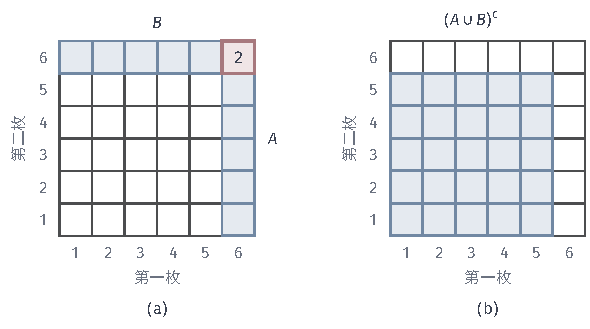
\includegraphics[width=100mm]{figures/07-probability/01-elementary-probability/tikz/cprob-at-least-one-six/figure.pdf}
  \caption{两枚骰子中至少一个六点。(a)浅蓝的一列是$A$（第一枚六点），浅蓝的一行是$B$（第二枚六点），红格$(6,6)$在$\lvert A\rvert+\lvert B\rvert$中被数了两次。(b)补事件“两枚都不是六点”是$5\times5$的方块。}
  \label{fig:cprob-at-least-one-six}
\end{BookInlineFigure}

用补事件计算更直接。由De Morgan律，$(A\cup B)^{\mathrm{c}}$就是$A^{\mathrm{c}}\cap B^{\mathrm{c}}$，即“两枚都不是六点”，即图~\ref{fig:cprob-at-least-one-six}(b)中$5\times5=25$个格子，所以概率是$1-25/36=11/36$，两种算法一致。

掷三枚骰子时两种方法的差别更明显。用式~\eqref{eq:cprob-inclusion-exclusion}，单个事件各占$36$个结果，两两之交各占$6$个，三者之交占$1$个，于是
\[
 \mathbb{P}(\text{至少一个六点})=\frac{3\times36-3\times6+1}{216}=\frac{91}{216}.
\]
用补事件，“三枚都不是六点”有$5^{3}=125$个结果，概率是$1-125/216=91/216$。补事件只需要一次计数，容斥原理需要逐层修正。

\paragraph{交事件}
交事件要求几个条件同时满足，一般要在样本空间中把两个条件一起数。在摸球问题的有序记录中，令$H_1$为“第一个是黑球”，$E$为“两个球颜色不同”。$H_1\cap E$就是“第一个黑、第二个白”，有$3\times2=6$个有序对，所以$\mathbb{P}(H_1\cap E)=6/20$。

此时$\mathbb{P}(H_1)=12/20$，$\mathbb{P}(E)=12/20$，二者相乘得$0.36$，并不等于$0.3$。交事件的概率一般不能由各自的概率相乘得到；什么时候可以相乘，是第~\ref{sec:cprob-independence}节的问题。

\paragraph{放回与不放回}
最后固定一个抽检问题，比较放回与不放回。一批$20$件产品中有$4$件次品，随机抽取$5$件检查。不放回时，每个$5$件子集等可能，“没有次品”要求$5$件都取自$16$件合格品：
\[
 \mathbb{P}_{\text{不放回}}(\text{没有次品})=\frac{\binom{16}{5}}{\binom{20}{5}}=\frac{4368}{15504}\approx0.2817.
\]
若改用不放回的有序记录，分子分母分别是$P(16,5)$和$P(20,5)$，比值不变。

放回时，每次都从全部$20$件中取，有序记录有$20^{5}$个等可能结果，其中每次都取到合格品的有$16^{5}$个：
\[
 \mathbb{P}_{\text{放回}}(\text{没有次品})=\Bigl(\frac{16}{20}\Bigr)^{5}=0.32768.
\]
放回时同一件合格品可以被反复抽到，合格品“用不完”，所以全是合格品的机会更大。

两种方式下“恰好一件次品”的计数方法不同。不放回时选$1$件次品、$4$件合格品，概率为
\[
 \frac{\binom41\binom{16}{4}}{\binom{20}{5}}=\frac{7280}{15504}\approx0.4696.
\]
放回时必须用有序记录：先选次品出现在哪一次，有$5$种；该次有$4$种取法，其余四次各有$16$种。于是概率为
\[
 \frac{5\times4\times16^{4}}{20^{5}}=0.4096.
\]
这里不能把放回的结果按无序组合来数，因为表~\ref{tab:cprob-sampling}最后一行的结果不等可能。

图~\ref{fig:cprob-replacement-compare}把“没有次品”的概率画成抽取件数$k$的函数。不放回的曲线始终低于放回的曲线，并在$k=17$时降到$0$：$17$件中至少有一件次品，因为合格品只有$16$件。$k$相对于$20$较小时两条曲线很接近，每次抽走一件对剩余构成的影响较小。

\begin{BookInlineFigure}
  \centering
  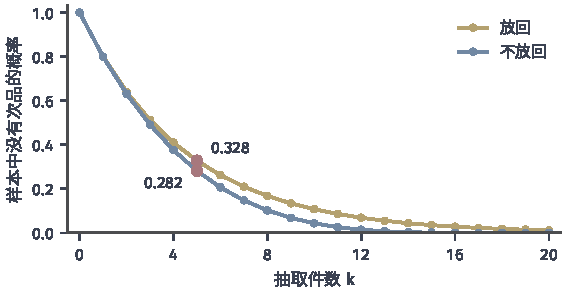
\includegraphics[width=96mm]{figures/07-probability/01-elementary-probability/matplotlib/cprob-replacement-compare/figure.pdf}
  \caption{$20$件中含$4$件次品时，抽取$k$件都是合格品的概率。蓝线是不放回抽样$\binom{16}{k}/\binom{20}{k}$，黄线是放回抽样$0.8^{k}$；红点标出正文中$k=5$的两个值。}
  \label{fig:cprob-replacement-compare}
\end{BookInlineFigure}

\section{条件概率}
\label{sec:cprob-conditional}

掷两枚骰子，第一枚是六点的概率是$1/6$。若有人看了一眼，告诉我们“点数和不小于$9$”，第一枚是六点的可能性还是$1/6$吗？直觉上应该更大，点数和大，说明骰子点数偏高。已知信息排除了一部分结果，剩余不确定性应当只在留下的结果中描述。

\paragraph{缩小范围，重新归一}
令$A$为“第一枚是六点”，$B$为“点数和不小于$9$”。$B$包含点数和为$9,10,11,12$的格子，个数分别是$4,3,2,1$，共$10$个；其中第一枚是六点的有$(6,3),(6,4),(6,5),(6,6)$这$4$个，如图~\ref{fig:cprob-conditioning-shrink}所示。

既然知道结果落在$B$中，$B$之外的$26$个格子就不必再考虑。原来$36$个结果等可能，留下的$10$个结果之间也没有理由偏向哪个，所以把它们看成新的等可能样本空间，每格的概率从$1/36$变为$1/10$。在这个缩小的范围里，$A$占$4$格，可能性是$4/10=2/5$。

\begin{BookInlineFigure}
  \centering
  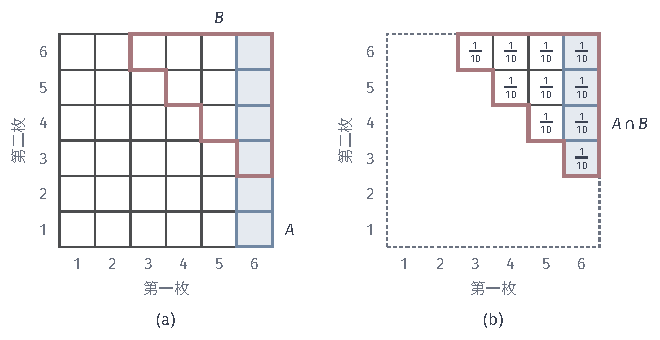
\includegraphics[width=112mm]{figures/07-probability/01-elementary-probability/tikz/cprob-conditioning-shrink/figure.pdf}
  \caption{以“点数和不小于$9$”为条件。(a)红线围出条件事件$B$的$10$个格子，浅蓝一列是$A$（第一枚六点），每格概率$1/36$。(b)只保留$B$中的格子，每格重新分得$1/10$；浅蓝格子是$A\cap B$，共$4$格，条件概率为$4/10$。}
  \label{fig:cprob-conditioning-shrink}
\end{BookInlineFigure}

把这个计算写成概率的形式。在古典模型中，
\[
 \frac{\lvert A\cap B\rvert}{\lvert B\rvert}
 =\frac{\lvert A\cap B\rvert/\lvert\Omega\rvert}{\lvert B\rvert/\lvert\Omega\rvert}
 =\frac{\mathbb{P}(A\cap B)}{\mathbb{P}(B)}.
\]
右端不再提到计数，只用到事件的概率，因此可以作为一般的定义。

\begin{definition}[条件概率]
\label{def:cprob-conditional}
设事件$B$满足$\mathbb{P}(B)>0$。事件$A$在$B$发生条件下的\term{条件概率}（conditional probability）定义为
\begin{equation}
 \mathbb{P}(A\mid B)=\frac{\mathbb{P}(A\cap B)}{\mathbb{P}(B)}.
 \label{eq:cprob-conditional}
\end{equation}
\end{definition}

分子只保留$A$中同时落在$B$内的部分，分母把$B$的概率重新标定为$1$。用质量的图景说：把$B$之外的质量全部清除，再把$B$内的质量按原有比例放大，使总量回到$1$。$B$内各点之间的相对大小不变，这正是“已知$B$发生”所允许的全部修改。

条件$\mathbb{P}(B)>0$不能去掉。在有限的古典模型中，$\mathbb{P}(B)=0$意味着$B=\varnothing$，以一个不可能发生的事件为条件没有意义，式~\eqref{eq:cprob-conditional}的分母也为零。

\paragraph{条件概率仍是概率}
固定$B$以后，$A\mapsto\mathbb{P}(A\mid B)$给每个事件分配了一个数。它满足前面的三条基本性质，因而第~\ref{sec:cprob-computing}节的补事件公式、加法公式在条件之下都可以照用。

\begin{theorem}[条件概率的基本性质]
\label{thm:cprob-conditional-axioms}
设$\mathbb{P}(B)>0$，则对任意事件$A,A'$，
\begin{equation}
 \mathbb{P}(A\mid B)\geq0,\qquad \mathbb{P}(\Omega\mid B)=1,
 \label{eq:cprob-conditional-normalized}
\end{equation}
并且当$A\cap A'=\varnothing$时，
\begin{equation}
 \mathbb{P}(A\cup A'\mid B)=\mathbb{P}(A\mid B)+\mathbb{P}(A'\mid B).
 \label{eq:cprob-conditional-additive}
\end{equation}
\end{theorem}

\begin{proof}
非负性来自分子非负、分母为正。由$\Omega\cap B=B$，分子分母相同，所以$\mathbb{P}(\Omega\mid B)=1$。若$A\cap A'=\varnothing$，则$A\cap B$与$A'\cap B$也互斥，且它们的并是$(A\cup A')\cap B$。由式~\eqref{eq:cprob-additive}，
\[
 \mathbb{P}\bigl((A\cup A')\cap B\bigr)=\mathbb{P}(A\cap B)+\mathbb{P}(A'\cap B).
\]
两边同除以$\mathbb{P}(B)$，就得到式~\eqref{eq:cprob-conditional-additive}。
\end{proof}

例如在上面的骰子例子中，$\mathbb{P}(A^{\mathrm{c}}\mid B)=1-2/5=3/5$，即已知点数和不小于$9$时，第一枚不是六点的概率是$3/5$。

\paragraph{两个方向的条件概率}
$\mathbb{P}(A\mid B)$与$\mathbb{P}(B\mid A)$的分子相同，都是$\mathbb{P}(A\cap B)$，分母不同。在骰子例子中，
\[
 \mathbb{P}(A\mid B)=\frac{4/36}{10/36}=\frac25,\qquad
 \mathbb{P}(B\mid A)=\frac{4/36}{6/36}=\frac23.
\]
前者是“点数和大时，第一枚是六点的概率”，后者是“第一枚是六点时，点数和大的概率”。它们回答不同的问题，一般不相等。把两者混为一谈是条件概率中最常见的错误，后面的检测例子会显示它可以造成多大的偏差。

已知$B$让$A$的概率从$1/6$升到$2/5$，这是信息的作用。条件概率也可能比原概率小，例如已知“点数和不大于$4$”时，第一枚是六点的概率降为$0$。若条件概率与原概率相等，条件就没有改变$A$的可能性，这种情形在第~\ref{sec:cprob-independence}节研究。

\subsection{乘法规则}
\label{sec:cprob-multiplication-rule}

很多试验是分步进行的：先摸第一个球，再摸第二个；先选产线，再看产品是否合格。每一步的条件概率往往可以直接从当时的物理状态读出，而整个样本空间却不必列出。把定义~\eqref{eq:cprob-conditional}反过来用，就能把这些逐步的概率乘起来。

\paragraph{两步乘法}
式~\eqref{eq:cprob-conditional}两边乘以$\mathbb{P}(B)$，得到
\begin{equation}
 \mathbb{P}(A\cap B)=\mathbb{P}(B)\,\mathbb{P}(A\mid B),\qquad \mathbb{P}(B)>0.
 \label{eq:cprob-multiplication}
\end{equation}
这称为概率的\term{乘法规则}（multiplication rule）。它的含义是比例的比例：$B$占全体的比例，乘以$A$在$B$内部所占的比例，等于$A\cap B$占全体的比例。

回到摸球问题，令$H_i$为“第$i$个球是黑球”。第一个球是黑球的概率是$3/5$。第一个黑球摸走以后，盒中剩下$2$黑$2$白，所以$\mathbb{P}(H_2\mid H_1)=2/4$。由式~\eqref{eq:cprob-multiplication}，
\[
 \mathbb{P}(H_1\cap H_2)=\mathbb{P}(H_1)\,\mathbb{P}(H_2\mid H_1)=\frac35\cdot\frac24=\frac{3}{10}.
\]
这与第~\ref{sec:cprob-computing}节在有序记录中数出的$6/20$一致。

这里的$\mathbb{P}(H_2\mid H_1)=2/4$是从“已知第一个是黑球”这个条件下盒中的实际构成读出来的。若忽略条件的变化，把第二步也写成$3/5$，就会得到$9/25$，那是放回摸球的答案。不放回抽样中，每一步的条件概率都必须对应前面已经发生的结果。

\paragraph{树形图}
把所有分步的情形画出来，就得到图~\ref{fig:cprob-urn-tree}的树形图。从根出发，每一层是一步，分支上写的是在到达该分支之前的结果已知时的条件概率；从根到叶的一条路径是一个完整的结果，它的概率是路径上各分支概率的乘积。

\begin{BookInlineFigure}
  \centering
  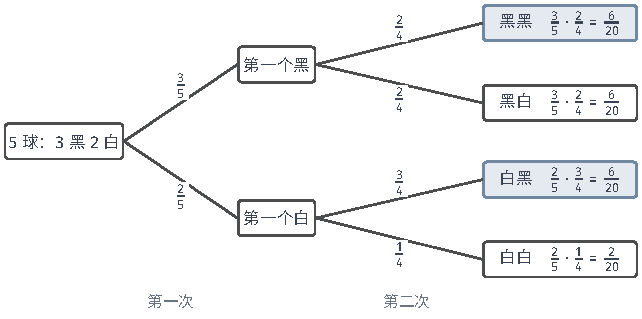
\includegraphics[width=109mm]{figures/07-probability/01-elementary-probability/tikz/cprob-urn-tree/figure.pdf}
  \caption{不放回摸两个球的树形图（盒中$3$黑$2$白）。分支上的数是条件概率，叶上是路径概率的乘积；四个叶的概率之和为$1$。浅蓝的两个叶组成事件$H_2$“第二个是黑球”。}
  \label{fig:cprob-urn-tree}
\end{BookInlineFigure}

同一个节点引出的分支，条件概率之和为$1$，这是式~\eqref{eq:cprob-conditional-normalized}的体现；因此全部叶的概率之和也是$1$。树形图上的叶就是颜色记录的四个结果，叶上的数与图~\ref{fig:cprob-urn-records}(c)一致。

\paragraph{多步乘法}
步骤更多时，反复使用式~\eqref{eq:cprob-multiplication}即可。

\begin{theorem}[多步乘法规则]
\label{thm:cprob-chain-rule}
设事件$A_1,\ldots,A_n$满足$\mathbb{P}(A_1\cap\cdots\cap A_{n-1})>0$，则
\begin{equation}
 \mathbb{P}(A_1\cap\cdots\cap A_n)
 =\mathbb{P}(A_1)\prod_{k=2}^{n}\mathbb{P}(A_k\mid A_1\cap\cdots\cap A_{k-1}).
 \label{eq:cprob-chain-rule}
\end{equation}
\end{theorem}

\begin{proof}
记$C_k=A_1\cap\cdots\cap A_k$。由包含关系$C_{n-1}\subseteq C_{n-2}\subseteq\cdots\subseteq C_1$与式~\eqref{eq:cprob-monotone}，各$\mathbb{P}(C_k)\geq\mathbb{P}(C_{n-1})>0$，右端每个条件概率都有定义。由定义~\eqref{eq:cprob-conditional}与$C_{k-1}\cap A_k=C_k$，
\[
 \mathbb{P}(A_k\mid C_{k-1})=\frac{\mathbb{P}(C_k)}{\mathbb{P}(C_{k-1})},\qquad k=2,\ldots,n,
\]
所以右端是
\[
 \mathbb{P}(C_1)\cdot\frac{\mathbb{P}(C_2)}{\mathbb{P}(C_1)}\cdot\frac{\mathbb{P}(C_3)}{\mathbb{P}(C_2)}\cdots\frac{\mathbb{P}(C_n)}{\mathbb{P}(C_{n-1})}.
\]
相邻的分子分母逐个相消，只剩$\mathbb{P}(C_n)$，即左端。
\end{proof}

用它重新计算第~\ref{sec:cprob-computing}节的扑克牌问题。令$R_k$为“第$k$张是红桃”。第一张是红桃的概率是$13/52$；已知第一张是红桃，剩下$51$张中有$12$张红桃；已知前两张都是红桃，剩下$50$张中有$11$张。由式~\eqref{eq:cprob-chain-rule}，
\[
 \mathbb{P}(R_1\cap R_2\cap R_3)=\frac{13}{52}\cdot\frac{12}{51}\cdot\frac{11}{50}=\frac{1716}{132600}=\frac{11}{850}.
\]
这与组合计数$\binom{13}{3}/\binom{52}{3}$的结果相同。组合计数一次数完整个样本空间，乘法规则则沿抽取过程逐步计算，每一步只需看当时剩下什么。

\subsection{全概率与Bayes公式}
\label{sec:cprob-total-bayes}

一家工厂有甲、乙、丙三条产线，某天生产的$1000$件产品中，甲线$500$件、乙线$300$件、丙线$200$件，次品分别有$10$件、$12$件、$20$件。从这$1000$件中随机抽一件，它是次品的概率是多少？如果它是次品，它最可能来自哪条产线？前一个问题按来源分组再合计，后一个问题从结果反推来源。

\paragraph{按情形分组}
令$L_1,L_2,L_3$分别为“抽到的产品来自甲、乙、丙线”，$D$为“抽到的是次品”。每件产品恰好来自一条产线，所以$L_1,L_2,L_3$两两互斥，并且它们的并是$\Omega$。这样一组事件称为样本空间的一个\term{划分}（partition）：每次试验中恰有一个$L_i$发生。

每条产线的比例和次品率可以直接读出：
\[
 \mathbb{P}(L_1)=0.5,\quad \mathbb{P}(L_2)=0.3,\quad \mathbb{P}(L_3)=0.2,
\]
\[
 \mathbb{P}(D\mid L_1)=\frac{10}{500}=0.02,\qquad
 \mathbb{P}(D\mid L_2)=\frac{12}{300}=0.04,
\]
\[
 \mathbb{P}(D\mid L_3)=\frac{20}{200}=0.10.
\]
要得到$\mathbb{P}(D)$，把$D$按来源切成三块，分别用乘法规则计算，再相加。

\begin{theorem}[全概率公式]
\label{thm:cprob-total-probability}
设$L_1,\ldots,L_m$是样本空间的一个划分，且每个$\mathbb{P}(L_i)>0$。则对任意事件$D$，
\begin{equation}
 \mathbb{P}(D)=\sum_{i=1}^{m}\mathbb{P}(L_i)\,\mathbb{P}(D\mid L_i).
 \label{eq:cprob-total-probability}
\end{equation}
\end{theorem}

\begin{proof}
由$L_1\cup\cdots\cup L_m=\Omega$，得$D=(D\cap L_1)\cup\cdots\cup(D\cap L_m)$；由$L_i$两两互斥，各块$D\cap L_i$也两两互斥。由有限个事件的互斥可加性，
\[
 \mathbb{P}(D)=\sum_{i=1}^{m}\mathbb{P}(D\cap L_i).
\]
对每一项用乘法规则~\eqref{eq:cprob-multiplication}，把$\mathbb{P}(D\cap L_i)$写成$\mathbb{P}(L_i)\mathbb{P}(D\mid L_i)$，代入即得。
\end{proof}

式~\eqref{eq:cprob-total-probability}称为\term{全概率公式}（law of total probability）。它是一个加权平均：各组的次品率$\mathbb{P}(D\mid L_i)$按各组所占的比例$\mathbb{P}(L_i)$加权。代入产线的数据，
\[
 \mathbb{P}(D)=0.5\times0.02+0.3\times0.04+0.2\times0.10=0.010+0.012+0.020=0.042.
\]
这正是$1000$件中次品所占的比例$42/1000$。

图~\ref{fig:cprob-line-mosaic}(a)把这个加权平均画成面积。单位正方形按产线比例分成三列，每列底部深色条的高度是该线的次品率，深色条的面积就是$\mathbb{P}(D\cap L_i)$，三块面积之和是$\mathbb{P}(D)$。

\begin{BookInlineFigure}
  \centering
  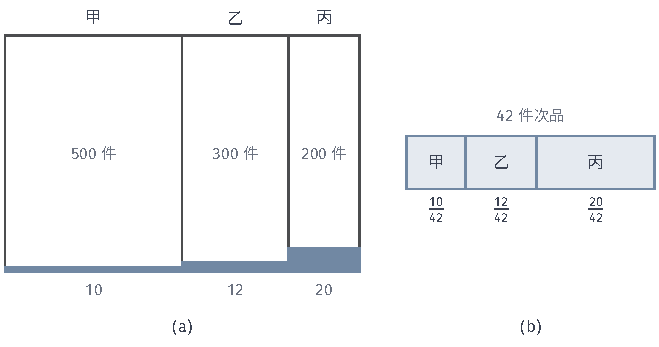
\includegraphics[width=112mm]{figures/07-probability/01-elementary-probability/tikz/cprob-line-mosaic/figure.pdf}
  \caption{三条产线的面积图，按真实比例绘制。(a)列宽是产线所占比例$0.5,0.3,0.2$，底部深蓝条的高度是次品率$0.02,0.04,0.10$，下方数字是各线次品件数；深蓝条的总面积是$\mathbb{P}(D)=0.042$。(b)只看$42$件次品，每件占同样长度，三段的比例就是$\mathbb{P}(L_i\mid D)$。}
  \label{fig:cprob-line-mosaic}
\end{BookInlineFigure}

\paragraph{从结果反推来源}
现在已知抽到的是次品，问它来自各条产线的概率。按定义，这是把范围缩小到$D$，在其中计算$L_i\cap D$所占的比例。分子用乘法规则写开，分母用全概率公式写开，就得到下面的公式。

\begin{theorem}[Bayes公式]
\label{thm:cprob-bayes}
在定理~\ref{thm:cprob-total-probability}的条件下，若$\mathbb{P}(D)>0$，则对每个$i$，
\begin{equation}
 \mathbb{P}(L_i\mid D)=\frac{\mathbb{P}(L_i)\,\mathbb{P}(D\mid L_i)}{\sum_{j=1}^{m}\mathbb{P}(L_j)\,\mathbb{P}(D\mid L_j)}.
 \label{eq:cprob-bayes}
\end{equation}
\end{theorem}

\begin{proof}
由定义~\eqref{eq:cprob-conditional}与乘法规则~\eqref{eq:cprob-multiplication}，
\[
 \mathbb{P}(L_i\mid D)=\frac{\mathbb{P}(L_i\cap D)}{\mathbb{P}(D)}=\frac{\mathbb{P}(L_i)\,\mathbb{P}(D\mid L_i)}{\mathbb{P}(D)}.
\]
再用全概率公式~\eqref{eq:cprob-total-probability}代入分母即得。
\end{proof}

式~\eqref{eq:cprob-bayes}称为\term{Bayes公式}（Bayes' formula）。分子就是图~\ref{fig:cprob-line-mosaic}(a)中第$i$块深色条的面积，分母是三块面积之和。代入数据，
\[
 \mathbb{P}(L_1\mid D)=\frac{0.010}{0.042}=\frac{10}{42},\quad
 \mathbb{P}(L_2\mid D)=\frac{12}{42},\quad
 \mathbb{P}(L_3\mid D)=\frac{20}{42}\approx0.476.
\]
在古典模型中这就是在$42$件次品里数各产线的件数，图~\ref{fig:cprob-line-mosaic}(b)把这$42$件单独排开。

\paragraph{先验与后验}
Bayes公式中的两组比例含义不同。$\mathbb{P}(L_i)$是抽到产品之前、不知道它是否为次品时对来源的估计，称为\term{先验}（prior）概率；$\mathbb{P}(L_i\mid D)$是观察到“次品”之后的来源概率，称为\term{后验}（posterior）概率。$\mathbb{P}(D\mid L_i)$是各来源产生这一观察的可能性。

丙线只生产了$20\%$的产品，却占了次品的约$47.6\%$；甲线生产了一半，在次品中只占约$23.8\%$。后验把先验按“各来源产生观察的可能性”重新加权：次品率高的产线，在次品中的份额被放大。

若要把这件次品归到一条产线去追查，按后验概率最大的原则应归到丙线。这是用条件概率作分类：比较的是$\mathbb{P}(L_i\mid D)$，而不是$\mathbb{P}(L_i)$或$\mathbb{P}(D\mid L_i)$单独一项。若抽到的是合格品，同样的计算给出后验约为$0.512,0.301,0.188$，与先验相差不大，合格品几乎不提供来源的信息。

条件也可以反推时间上更早的结果。在摸球问题中，已知第二个球是黑球，第一个球是黑球的概率是多少？由图~\ref{fig:cprob-urn-tree}，$\mathbb{P}(H_2)=6/20+6/20=3/5$，于是
\[
 \mathbb{P}(H_1\mid H_2)=\frac{\mathbb{P}(H_1\cap H_2)}{\mathbb{P}(H_2)}=\frac{6/20}{12/20}=\frac12.
\]
第二个球不能影响第一个球是什么，但知道第二个球的颜色，会改变我们对第一个球的判断。条件概率描述的是信息，而不是因果。

\paragraph{条件要对应实际得到的信息}
用条件概率时，条件必须是实际知道的那个事件，而不是与它意思相近的另一个事件。下面的三扇门问题说明两者的差别。三扇门中的一扇后面有奖品，奖品在各扇门后的可能性相同。参赛者选了1号门；主持人知道奖品的位置，他从另外两扇门中打开一扇没有奖品的门，若两扇都没有奖品，就各以$1/2$的概率任选一扇。现在主持人打开了3号门，奖品在2号门后的概率是多少？

一种常见的回答是：3号门后没有奖品，剩下1号和2号两扇门，各占$1/2$。这个回答所用的条件是“奖品不在3号门后”，可我们实际看到的是“主持人打开了3号门”。后者比前者包含更多信息：奖品若在1号门后，主持人有两扇门可选；奖品若在2号门后，他只能打开3号门。

令$C_i$为“奖品在$i$号门后”，$O_3$为“主持人打开3号门”。$C_1,C_2,C_3$构成划分，各自的先验概率是$1/3$。由主持人的规则，
\[
 \mathbb{P}(O_3\mid C_1)=\frac12,\qquad \mathbb{P}(O_3\mid C_2)=1,\qquad \mathbb{P}(O_3\mid C_3)=0.
\]
由全概率公式与Bayes公式，
\[
 \mathbb{P}(O_3)=\frac13\Bigl(\frac12+1+0\Bigr)=\frac12,
\]
\[
 \mathbb{P}(C_2\mid O_3)=\frac{\frac13\cdot1}{\frac12}=\frac23,\qquad
 \mathbb{P}(C_1\mid O_3)=\frac{\frac13\cdot\frac12}{\frac12}=\frac13.
\]

图~\ref{fig:cprob-three-doors-tree}把四种情形画成树形图。红框的两片叶是“打开3号门”，它们的概率分别是$1/6$和$1/3$，后者是前者的两倍。所以换到2号门，得到奖品的概率是$2/3$。若主持人并不知道奖品位置、只是碰巧打开了一扇空门，$\mathbb{P}(O_3\mid C_2)$就变成$1/2$，答案也随之变成$1/2$。同样是“3号门后没有奖品”，信息产生的方式不同，条件事件就不同。

\begin{BookInlineFigure}
  \centering
  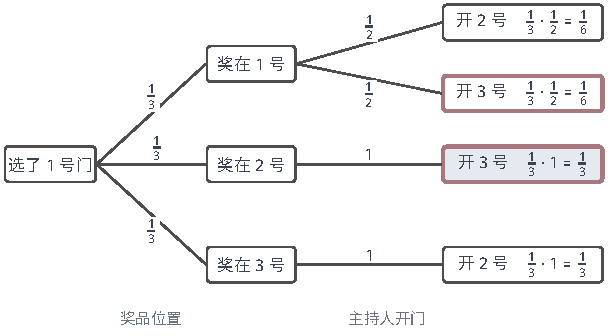
\includegraphics[width=103mm]{figures/07-probability/01-elementary-probability/tikz/cprob-three-doors-tree/figure.pdf}
  \caption{三扇门问题的树形图。第一层是奖品位置，第二层是主持人按规则开的门，分支上是条件概率，叶上是路径概率。红框的两片叶组成观察到的事件“打开3号门”，其中浅蓝的一片（奖在2号门后）占$\frac{1/3}{1/2}=\frac23$。}
  \label{fig:cprob-three-doors-tree}
\end{BookInlineFigure}

\paragraph{检测中的三个比例}
产品出厂前要经过一道自动检测。设某批产品中次品率为$2\%$；检测对次品报警的概率为$0.95$，对合格品误报的概率为$0.05$。一件产品报警了，它是次品的概率是多少？很多人会回答$0.95$，下面的计算说明这个答案错得很远。

令$D$为“次品”，$T$为“报警”。已知量是
\[
 \mathbb{P}(D)=0.02,\qquad \mathbb{P}(T\mid D)=0.95,\qquad \mathbb{P}(T\mid D^{\mathrm{c}})=0.05.
\]
$D$与$D^{\mathrm{c}}$构成划分。由全概率公式，报警的概率是
\[
 \mathbb{P}(T)=0.02\times0.95+0.98\times0.05=0.019+0.049=0.068.
\]
由Bayes公式，
\[
 \mathbb{P}(D\mid T)=\frac{0.019}{0.068}=\frac{19}{68}\approx0.279.
\]

图~\ref{fig:cprob-test-frequency-tree}用$10000$件产品把这些比例换成件数。$200$件次品中有$190$件报警，$9800$件合格品中有$490$件误报；报警的$680$件里只有$190$件是次品。误报率虽小，合格品的数量却大得多，误报的件数反而超过了真正的次品。

\begin{BookInlineFigure}
  \centering
  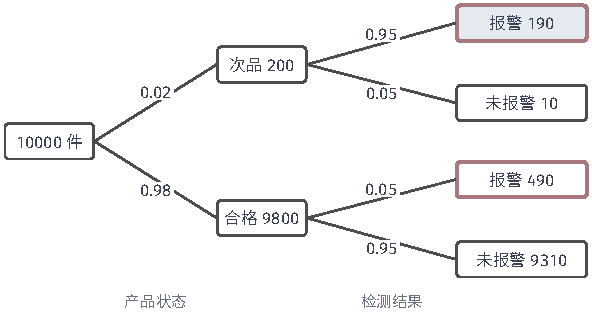
\includegraphics[width=100mm]{figures/07-probability/01-elementary-probability/tikz/cprob-test-frequency-tree/figure.pdf}
  \caption{用$10000$件产品表示检测的各个比例。分支上的数是条件概率，节点中是件数；红框是报警的两组，浅蓝的一组是报警且为次品，占报警件数的$190/680\approx0.279$。}
  \label{fig:cprob-test-frequency-tree}
\end{BookInlineFigure}

这个例子中三个数分别回答三个问题：先验比例$\mathbb{P}(D)=0.02$是检测前一件产品为次品的概率；条件检出概率$\mathbb{P}(T\mid D)=0.95$描述检测的性能，即在次品中报警的比例；后验比例$\mathbb{P}(D\mid T)\approx0.279$是在报警的产品中次品的比例。第二个与第三个的分子相同、分母不同，正是前面说的两个方向的条件概率。

\paragraph{信息的逐次更新}
报警的产品再送去复检一次。设复检用同样性能的设备，并假设：对给定状态的产品，复检是否报警不受第一次结果的影响，即
\[
 \mathbb{P}(T_2\mid D\cap T_1)=\mathbb{P}(T_2\mid D)=0.95,\qquad
 \mathbb{P}(T_2\mid D^{\mathrm{c}}\cap T_1)=\mathbb{P}(T_2\mid D^{\mathrm{c}})=0.05,
\]
其中$T_1,T_2$分别是两次报警。若两次报警之后才判定，次品的概率是多少？

已知$T_1$发生，就在$\mathbb{P}(\cdot\mid T_1)$下计算。由定理~\ref{thm:cprob-conditional-axioms}，它满足三条基本性质，所以全概率公式与Bayes公式对它同样成立。在它之下再以$D$为条件，得到的正是以$D\cap T_1$为条件：
\[
 \frac{\mathbb{P}(T_2\cap D\mid T_1)}{\mathbb{P}(D\mid T_1)}
 =\frac{\mathbb{P}(T_2\cap D\cap T_1)/\mathbb{P}(T_1)}{\mathbb{P}(D\cap T_1)/\mathbb{P}(T_1)}
 =\mathbb{P}(T_2\mid D\cap T_1).
\]
因此公式中的先验换成第一次报警后的后验$19/68$，条件检出概率换成上面假设的$\mathbb{P}(T_2\mid D\cap T_1)$与$\mathbb{P}(T_2\mid D^{\mathrm{c}}\cap T_1)$：
\[
 \mathbb{P}(D\mid T_1\cap T_2)
 =\frac{\frac{19}{68}\times0.95}{\frac{19}{68}\times0.95+\frac{49}{68}\times0.05}
 =\frac{18.05}{18.05+2.45}=\frac{361}{410}\approx0.880.
\]
一次观察后的后验成为下一次观察的先验，信息就这样逐次累积。

比值的写法更能看出每次更新做了什么。次品与合格品的概率之比，先验是$0.02:0.98=1:49$。由式~\eqref{eq:cprob-bayes}，两个后验的分母相同，比值只由分子决定：
\begin{equation}
 \frac{\mathbb{P}(D\mid T)}{\mathbb{P}(D^{\mathrm{c}}\mid T)}
 =\frac{\mathbb{P}(D)}{\mathbb{P}(D^{\mathrm{c}})}\cdot\frac{\mathbb{P}(T\mid D)}{\mathbb{P}(T\mid D^{\mathrm{c}})}.
 \label{eq:cprob-odds}
\end{equation}
右端第二个因子称为观察$T$的\term{似然比}（likelihood ratio），这里是$0.95/0.05=19$。每次报警把比值乘以$19$：一次后为$19:49$，即概率$19/68$；两次后为$361:49$，即概率$361/410$。

图~\ref{fig:cprob-posterior-prior}把后验画成先验次品率的函数。先验很小时，一次报警之后的后验仍然不大；同一个似然比作用在不同的先验上，结果可以相差很多。这再次说明，只知道检测的性能，不知道先验比例，无法回答“报警的产品有多大可能是次品”。

\begin{BookInlineFigure}
  \centering
  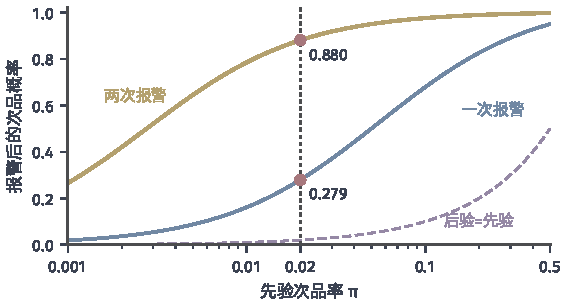
\includegraphics[width=96mm]{figures/07-probability/01-elementary-probability/matplotlib/cprob-posterior-prior/figure.pdf}
  \caption{报警后为次品的概率随先验次品率$\pi$的变化，横轴为对数坐标。检出概率$0.95$，误报概率$0.05$。蓝线是一次报警后的后验，黄线是两次报警后的后验（假设给定状态时两次检测互不影响），紫色虚线是后验等于先验的参考线；红点标出正文中$\pi=0.02$的两个值。}
  \label{fig:cprob-posterior-prior}
\end{BookInlineFigure}

两次更新所用的假设必须核对。如果某类次品的缺陷检测设备根本看不出来，第一次漏报的产品第二次也会漏报，两次结果就不再互不影响，乘以两次似然比会高估证据的强度。这个假设是对条件概率$\mathbb{P}(\cdot\mid D)$与$\mathbb{P}(\cdot\mid D^{\mathrm{c}})$的要求，下一节会看到它与“两次报警互不影响”并不是一回事。

\section{事件的独立性}
\label{sec:cprob-independence}

不放回摸球时，第一个球的颜色改变了第二个球的概率：$\mathbb{P}(H_2\mid H_1)=1/2$，而$\mathbb{P}(H_2)=3/5$。放回摸球时，第一个球摸出后又放了回去，盒中构成不变，无论第一个是什么颜色，第二个是黑球的概率都是$3/5$。在后一种情形下，知道第一个结果不提供关于第二个结果的任何信息，计算交事件的概率时可以把两个概率直接相乘。怎样把“不提供信息”准确地写出来？

\paragraph{定义}
放回摸球的有序记录有$25$个等可能结果，其中两个都是黑球的有$3\times3=9$个，所以
\[
 \mathbb{P}(H_2\mid H_1)=\frac{9/25}{15/25}=\frac35=\mathbb{P}(H_2).
\]
条件概率等于原来的概率，就是“已知$H_1$不改变$H_2$的可能性”。把等式$\mathbb{P}(H_2\mid H_1)=\mathbb{P}(H_2)$乘以$\mathbb{P}(H_1)$，得到一个对两个事件对称的乘积形式，并且在条件事件概率为零时也有意义。

\begin{definition}[两个事件的独立]
\label{def:cprob-independent}
若事件$A,B$满足
\begin{equation}
 \mathbb{P}(A\cap B)=\mathbb{P}(A)\,\mathbb{P}(B),
 \label{eq:cprob-independent}
\end{equation}
就称$A$与$B$\term{独立}（independent）。
\end{definition}

当$\mathbb{P}(B)>0$时，由定义~\eqref{eq:cprob-conditional}，式~\eqref{eq:cprob-independent}等价于$\mathbb{P}(A\mid B)=\mathbb{P}(A)$；当$\mathbb{P}(A)>0$时，它也等价于$\mathbb{P}(B\mid A)=\mathbb{P}(B)$。所以独立是对称的：$B$不提供关于$A$的信息，$A$也不提供关于$B$的信息。

\paragraph{独立是数量关系}
独立性要按式~\eqref{eq:cprob-independent}核对，不能凭“看起来有没有关系”判断。从一副$52$张的牌中抽一张，令$A$为“抽到A”，$B$为“抽到红桃”。四张A中恰有一张红桃，所以
\[
 \mathbb{P}(A\cap B)=\frac{1}{52},\qquad
 \mathbb{P}(A)\,\mathbb{P}(B)=\frac{4}{52}\cdot\frac{13}{52}=\frac{1}{52}.
\]
二者独立。原因在于一副牌是$13$种点数与$4$种花色的全部搭配，每种点数在各花色中出现的比例都相同。

掷两枚骰子，令$A$为“第一枚是偶数”，$C$为“点数和为$7$”，$D$为“点数和为$8$”。点数和要用到第一枚的点数，似乎不会与$A$独立。在图~\ref{fig:cprob-independence-grid}(a)中数一数：$A$占$18$格，$C$的$6$格中有$3$格落在$A$里，所以
\[
 \mathbb{P}(A\cap C)=\frac{3}{36}=\frac12\cdot\frac16=\mathbb{P}(A)\,\mathbb{P}(C).
\]
$A$与$C$独立。原因是对第一枚的每个点数$i$，第二枚都恰有一个点数$7-i$使和为$7$，和为$7$的比例在每一列中都是$1/6$。

\begin{BookInlineFigure}
  \centering
  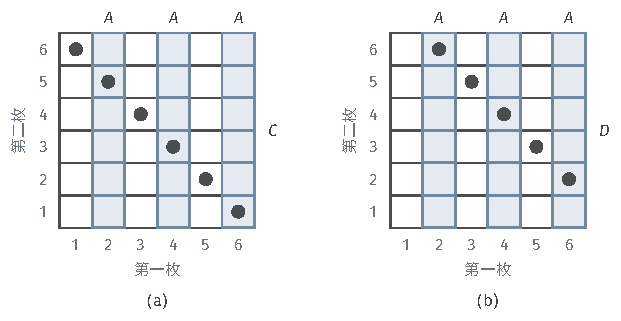
\includegraphics[width=105mm]{figures/07-probability/01-elementary-probability/tikz/cprob-independence-grid/figure.pdf}
  \caption{同一事件$A$（浅蓝三列，第一枚为偶数）与两个事件的关系。(a)圆点是$C$（点数和为$7$），在$A$内外各占所在列的$1/6$，$A$与$C$独立。(b)圆点是$D$（点数和为$8$），$A$内有$3$个、$A$外只有$2$个，$A$与$D$不独立。}
  \label{fig:cprob-independence-grid}
\end{BookInlineFigure}

$D$的情形不同。和为$8$的格子是$(2,6),(3,5),(4,4),(5,3),(6,2)$，其中第一枚为偶数的有$3$个，见图~\ref{fig:cprob-independence-grid}(b)。于是
\[
 \mathbb{P}(A\cap D)=\frac{3}{36},\qquad \mathbb{P}(A)\,\mathbb{P}(D)=\frac12\cdot\frac{5}{36}=\frac{2.5}{36}.
\]
两者不等，$A$与$D$不独立：第一枚为$1$时第二枚不可能凑出$8$，所以$D$在$A$之外的比例较低。对比$C$与$D$，事件之间在物理上是否“有关”不决定独立性，决定它的是交事件的比例。

\paragraph{独立与互斥}
互斥和独立都描述两个事件的关系，含义却几乎相反。互斥是集合之间的关系：$A\cap B=\varnothing$，两个事件不能同时发生，它与概率如何分配无关。独立是概率之间的关系：一个事件发生与否不改变另一个的概率，它取决于$\mathbb{P}$。

设$\mathbb{P}(A)>0$，$\mathbb{P}(B)>0$，且$A$与$B$互斥，则
\[
 \mathbb{P}(A\cap B)=0<\mathbb{P}(A)\,\mathbb{P}(B),
\]
二者不独立。这很合理：知道$B$发生，就确知$A$没有发生，$B$提供了关于$A$的完全信息。只有当其中一个事件的概率为零时，互斥的两个事件才独立。

\paragraph{补事件保持独立}
若$B$发生不提供关于$A$的信息，那么$B$不发生也不应提供信息。下面先对两个事件证实这一点，相互独立的多个事件在下一段定义之后再作推广。

\begin{theorem}[独立与补事件]
\label{thm:cprob-independent-complement}
若$A$与$B$独立，则$A$与$B^{\mathrm{c}}$独立，$A^{\mathrm{c}}$与$B$独立，$A^{\mathrm{c}}$与$B^{\mathrm{c}}$也独立。
\end{theorem}

\begin{proof}
$A$是互斥的$A\cap B$与$A\cap B^{\mathrm{c}}$之并，由互斥可加性与独立性，
\[
 \mathbb{P}(A\cap B^{\mathrm{c}})=\mathbb{P}(A)-\mathbb{P}(A\cap B)=\mathbb{P}(A)\bigl(1-\mathbb{P}(B)\bigr)=\mathbb{P}(A)\,\mathbb{P}(B^{\mathrm{c}}).
\]
所以$A$与$B^{\mathrm{c}}$独立。交换$A,B$的角色得到第二个结论；对独立的$A^{\mathrm{c}}$与$B$再用一次第一个结论，得到第三个。
\end{proof}

\paragraph{多个事件的相互独立}
三个或更多事件时，“互不提供信息”的要求更强：不仅任意两个之间不提供信息，任意几个事件的发生情况也不应改变其余事件的概率。这需要对所有子组都验证乘积关系。

\begin{definition}[相互独立]
\label{def:cprob-mutually-independent}
称事件$A_1,\ldots,A_n$\term{相互独立}（mutually independent），若对任意$2\leq k\leq n$和任意下标$1\leq i_1<\cdots<i_k\leq n$，都有
\begin{equation}
 \mathbb{P}(A_{i_1}\cap\cdots\cap A_{i_k})=\mathbb{P}(A_{i_1})\cdots\mathbb{P}(A_{i_k}).
 \label{eq:cprob-mutually-independent}
\end{equation}
若只要求$k=2$的情形，即任意两个事件独立，就称它们\term{两两独立}（pairwise independent）。
\end{definition}

两两独立不能推出相互独立。抛两枚均匀硬币，四个有序结果等可能。令$A$为“第一枚正面”，$B$为“第二枚正面”，$C$为“两枚结果相同”。每个事件的概率都是$1/2$；由图~\ref{fig:cprob-two-coins-pairwise}，任意两个事件恰好共有一个结果，所以每对的交的概率都是$1/4=(1/2)^2$，三对都独立。

\begin{BookInlineFigure}
  \centering
  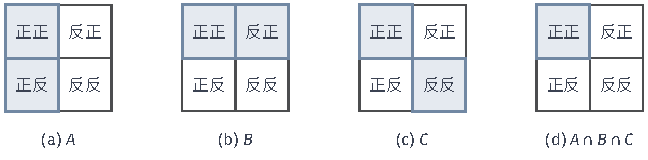
\includegraphics[width=110mm]{figures/07-probability/01-elementary-probability/tikz/cprob-two-coins-pairwise/figure.pdf}
  \caption{抛两枚硬币的四个等可能结果，“正反”表示第一枚正面、第二枚反面。浅蓝格子依次是(a)$A$：第一枚正面；(b)$B$：第二枚正面；(c)$C$：两枚相同；(d)$A\cap B\cap C$。任意两个事件的交都只有“正正”一格，三者之交也只有这一格。}
  \label{fig:cprob-two-coins-pairwise}
\end{BookInlineFigure}

但三个事件同时发生就是“正正”，于是
\[
 \mathbb{P}(A\cap B\cap C)=\frac14\neq\frac18=\mathbb{P}(A)\,\mathbb{P}(B)\,\mathbb{P}(C).
\]
三者不相互独立。原因很清楚：知道$A$与$B$都发生，就完全知道了$C$；单独知道其中任何一个，却对另一个毫无帮助。

反过来，只验证三者之交的乘积关系也不够。掷两枚骰子，令$E_1$为“第一枚是$1,2,3$之一”，$E_2$为“第一枚是$3,4,5$之一”，$E_3$为“点数和为$9$”。$E_1\cap E_2\cap E_3$只有结果$(3,6)$，于是
\[
 \mathbb{P}(E_1\cap E_2\cap E_3)=\frac{1}{36}=\frac12\cdot\frac12\cdot\frac19.
\]
然而$E_1\cap E_2$是“第一枚是$3$”，概率$1/6\neq1/4$，这两个事件不独立。定义~\ref{def:cprob-mutually-independent}要求所有子组的乘积关系，任何一层都不能省略。

\paragraph{多个事件的补}
定理~\ref{thm:cprob-independent-complement}可以推广到相互独立的多个事件：把其中任意几个换成补事件，所得的事件仍相互独立。只需说明换掉一个即可，换多个时逐个替换。设$A_1,\ldots,A_n$相互独立，把$A_1$换成$A_1^{\mathrm{c}}$。对含下标$1$的子组，记其余事件之交为$F$。由于$A_1,\ldots,A_n$的乘积关系对每个子组成立，$\mathbb{P}(F)$等于其余各事件概率之积，并且
\[
 \mathbb{P}(A_1\cap F)=\mathbb{P}(A_1)\,\mathbb{P}(F).
\]
重复定理~\ref{thm:cprob-independent-complement}的证明，得到
\[
 \mathbb{P}(A_1^{\mathrm{c}}\cap F)=\mathbb{P}(F)-\mathbb{P}(A_1\cap F)=\mathbb{P}(A_1^{\mathrm{c}})\,\mathbb{P}(F).
\]
不含下标$1$的子组不受影响，所以式~\eqref{eq:cprob-mutually-independent}对新的一组事件仍成立。

\paragraph{重复试验中的独立性从哪里来}
“两次投掷互不影响”这句话，在模型中究竟对应什么？以两枚骰子为例，样本空间是乘积$\Omega=\Omega_1\times\Omega_2$，$\Omega_1=\Omega_2=\{1,\ldots,6\}$，第~\ref{sec:cprob-equally-likely}节假设这$36$个有序对同样可能。只与第一枚有关的事件形如$A_1\times\Omega_2$，只与第二枚有关的事件形如$\Omega_1\times A_2$，它们的交是矩形$A_1\times A_2$，如图~\ref{fig:cprob-product-space}所示。

\begin{BookInlineFigure}
  \centering
  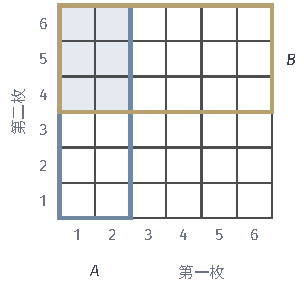
\includegraphics[width=53mm]{figures/07-probability/01-elementary-probability/tikz/cprob-product-space/figure.pdf}
  \caption{乘积样本空间中的独立性。蓝框是$A$：第一枚为$1$或$2$；黄框是$B$：第二枚为$4,5,6$之一。交$A\cap B$是$2\times3$的浅蓝矩形，其格数等于两边格数之积。}
  \label{fig:cprob-product-space}
\end{BookInlineFigure}

\begin{theorem}[乘积样本空间上的独立性]
\label{thm:cprob-product-independence}
设$\Omega=\Omega_1\times\cdots\times\Omega_n$，各$\Omega_k$有限且非空，$\Omega$上的全部结果同样可能。对每个$k$取$A_k\subseteq\Omega_k$，令
\begin{equation}
 E_k=\{(\omega_1,\ldots,\omega_n)\in\Omega:\ \omega_k\in A_k\}
 \label{eq:cprob-coordinate-event}
\end{equation}
为只与第$k$个分量有关的事件。则$E_1,\ldots,E_n$相互独立，并且
\begin{equation}
 \mathbb{P}(E_k)=\frac{\lvert A_k\rvert}{\lvert\Omega_k\rvert}.
 \label{eq:cprob-product-marginal}
\end{equation}
\end{theorem}

\begin{proof}
任取下标集合$S\subseteq\{1,\ldots,n\}$。按式~\eqref{eq:cprob-coordinate-event}，$\bigcap_{k\in S}E_k$由第$k$个分量在$A_k$中（$k\in S$）、其余分量任意的结果组成，它是乘积集合，各分量的取值范围分别是$A_k$（$k\in S$）或$\Omega_k$（$k\notin S$）。由乘法规则计数，
\[
 \Bigl\lvert\bigcap_{k\in S}E_k\Bigr\rvert=\prod_{k\in S}\lvert A_k\rvert\prod_{k\notin S}\lvert\Omega_k\rvert.
\]
$\Omega$本身也是乘积集合，$\lvert\Omega\rvert$等于各$\lvert\Omega_k\rvert$之积。两式相除，得到
\[
 \mathbb{P}\Bigl(\bigcap_{k\in S}E_k\Bigr)=\prod_{k\in S}\frac{\lvert A_k\rvert}{\lvert\Omega_k\rvert}.
\]
取$S=\{k\}$即得式~\eqref{eq:cprob-product-marginal}；把它代回上式，对每个至少含两个下标的$S$都得到式~\eqref{eq:cprob-mutually-independent}。
\end{proof}

定理说明，重复试验中的独立性是乘积样本空间上等可能假设的推论。这个假设比“每次试验各自等可能”更多：它还要求各次结果的每种搭配同样可能，这正是“互不影响”在模型中的含义。放回摸球的$25$个有序对是$\{1,\ldots,5\}\times\{1,\ldots,5\}$的全部，满足定理的条件，所以$H_1$与$H_2$独立。

不放回摸球的样本空间去掉了对角线，不再是乘积集合，定理不适用；实际计算也表明$\mathbb{P}(H_1\cap H_2)=3/10$，而$\mathbb{P}(H_1)\,\mathbb{P}(H_2)=9/25$，二者不独立。每一次单独看，第二个球在五个球中仍是等可能的，$\mathbb{P}(H_2)=3/5$；不独立来自两次之间的搭配受到限制。

\paragraph{至少成功一次}
独立性使“$n$次重复中至少成功一次”的计算变得简单。设每次试验中某事件发生的概率为$p$，各次的事件相互独立。由上面关于补事件的推广，各次“不发生”的事件也相互独立，所以$n$次都不发生的概率是$(1-p)^{n}$，于是
\begin{equation}
 \mathbb{P}(\text{至少发生一次})=1-(1-p)^{n}.
 \label{eq:cprob-at-least-once}
\end{equation}

一个经典的比较是：掷一枚骰子$4$次至少出现一个六点，与掷两枚骰子$24$次至少出现一次双六，哪个更可能？前者$p=1/6$，后者$p=1/36$，由式~\eqref{eq:cprob-at-least-once}，
\[
 1-\Bigl(\frac56\Bigr)^{4}\approx0.5177,\qquad
 1-\Bigl(\frac{35}{36}\Bigr)^{24}\approx0.4914.
\]
虽然$4/6=24/36$，两者却一个略大于一半、一个略小于一半。图~\ref{fig:cprob-repeated-trials}画出两条曲线：概率不是随次数线性增长，而是以$1-(1-p)^{n}$的形式逐渐接近$1$，“机会乘以次数”只在$np$很小时近似成立。

\begin{BookInlineFigure}
  \centering
  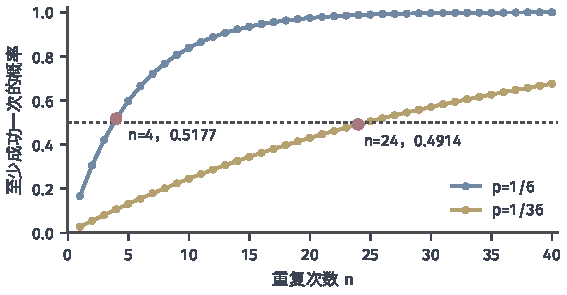
\includegraphics[width=96mm]{figures/07-probability/01-elementary-probability/matplotlib/cprob-repeated-trials/figure.pdf}
  \caption{$n$次独立重复中至少成功一次的概率$1-(1-p)^{n}$。蓝线$p=1/6$（一枚骰子出六点），黄线$p=1/36$（两枚骰子出双六），黑色点线是$1/2$；红点标出$n=4$与$n=24$两个值。}
  \label{fig:cprob-repeated-trials}
\end{BookInlineFigure}

同样的论证给出：$n$次中指定的$k$次成功、其余失败的概率是$p^{k}(1-p)^{n-k}$。在古典模型中$p$只能是有理数，例如$1/6$；成功次数的完整分布以及一般的$p$在第~\ref{chap:common-distributions}章讨论。

\paragraph{条件之下的独立}
回到第~\ref{sec:cprob-total-bayes}节的复检。那里假设的是：对次品，两次检测是否报警互不影响；对合格品也是如此。用本节的语言，就是$T_1$与$T_2$在条件概率$\mathbb{P}(\cdot\mid D)$下独立，在$\mathbb{P}(\cdot\mid D^{\mathrm{c}})$下也独立：
\[
 \mathbb{P}(T_1\cap T_2\mid D)=0.95^{2},\qquad
 \mathbb{P}(T_1\cap T_2\mid D^{\mathrm{c}})=0.05^{2}.
\]

不按状态区分时，$T_1$与$T_2$并不独立。由全概率公式，
\[
 \mathbb{P}(T_1\cap T_2)=0.02\times0.9025+0.98\times0.0025=0.0205,
\]
而两次报警各自的概率都是$0.068$，乘积为
\[
 \mathbb{P}(T_1)\,\mathbb{P}(T_2)=0.068^{2}\approx0.0046.
\]第一次报警提高了产品是次品的可能性，从而提高了第二次报警的可能性，两次报警通过产品的状态联系在一起。条件之下的独立与不加条件的独立是两回事，一般理论在第~\ref{chap:conditional-distributions}章建立。

\section{模型的适用范围}
\label{sec:cprob-scope}

古典模型的全部计算都建立在一个前提上：样本空间有限，每个样本点同样可能。前面几节一再看到，同一个试验换一种记录方式，这个前提就可能不再成立。本节把失效的情形归为三类：记录合并了不等量的基本结果、结果有无穷多个、结果取连续的位置。对每一类，我们说明计数比为什么失效，以及后面的章节用什么代替它。

\paragraph{合并后的结果}
掷两枚骰子，如果只记录出现了哪两个点数而不分先后，结果就是可重复的无序对，例如$\{1,1\}$、$\{1,2\}$、$\{3,5\}$。由表~\ref{tab:cprob-sampling}最后一行，这样的结果共有$\binom{6+2-1}{2}=21$个。它们是否同样可能？

图~\ref{fig:cprob-merged-classes}显示了每个无序结果合并了哪些有序结果。对角线上的$\{i,i\}$只对应一个有序对$(i,i)$，概率是$1/36$；其余的$\{i,j\}$（$i\neq j$）对应关于对角线对称的两个格子$(i,j)$与$(j,i)$，概率是$2/36$。$6$个一类、$15$个另一类，验证总和：
\[
 6\times\frac{1}{36}+15\times\frac{2}{36}=\frac{36}{36}=1.
\]

\begin{BookInlineFigure}
  \centering
  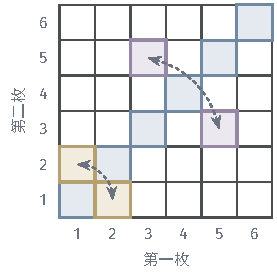
\includegraphics[width=47mm]{figures/07-probability/01-elementary-probability/tikz/cprob-merged-classes/figure.pdf}
  \caption{不记次序时两枚骰子的结果。浅蓝的对角线格子各自构成一个无序结果$\{i,i\}$；其余无序结果各由关于对角线对称的两个格子组成，黄色一对是$\{1,2\}$，紫色一对是$\{3,5\}$，虚线连接同一结果的两个格子。}
  \label{fig:cprob-merged-classes}
\end{BookInlineFigure}

若直接在$21$个无序结果上数，“两枚点数相同”占$6$个，会得到$6/21=2/7$；正确的答案是$6/36=1/6$。错误不在于用无序记录，而在于把合并了不同数量基本结果的类别当成了等可能的点。

一般地，若一个结果$r$是若干个等可能基本结果合并而成的，它的概率等于所合并的基本结果的概率之和。合并的个数不同，各结果的概率就不同。这时仍可以计算，但要给每个结果单独记一个概率$p(r)\geq0$，所有$p(r)$之和为$1$，事件的概率是它所含结果的$p(r)$之和。摸球的颜色记录、点数和、无序的点数对都属于这种情形，第~\ref{sec:cprob-equally-likely}节的三条基本性质对这样的分配仍然成立。

有些试验根本没有一个等可能的细化。一枚重心偏移的骰子，六个面朝上的机会本来就不同，无论怎样细分记录都找不到对称性。古典模型对它无能为力，只能直接给六个面各指定一个概率。给有限或可数个结果逐一指定概率的方式称为概率表，它在第~\ref{chap:random-variables}章与随机变量一起建立。

\paragraph{无穷多个结果}
抛一枚均匀硬币，直到第一次出现正面为止，记下所抛的次数。结果可以是$1,2,3,\ldots$中的任何一个，样本空间$\Omega=\{1,2,3,\ldots\}$有无穷多个点。

这些结果不可能同样可能。若每个结果的概率都是同一个数$c$，那么$c>0$时，任意取$N>1/c$个结果，它们的概率之和就超过$1$；$c=0$时，所有结果的概率都是零，总和无法是$1$。计数比$\lvert A\rvert/\lvert\Omega\rvert$在这里更没有意义，分母是无穷。

各结果的概率可以从有限的古典模型中算出。“第一次正面出现在第$k$次”只与前$k$次有关，它要求前$k-1$次都是反面、第$k$次是正面。前$k$次的$2^{k}$个有序结果等可能，满足要求的只有一个，所以
\begin{equation}
 \mathbb{P}(\text{第一次正面出现在第}k\text{次})=\frac{1}{2^{k}},\qquad k=1,2,\ldots.
 \label{eq:cprob-first-head}
\end{equation}

图~\ref{fig:cprob-first-head}(a)画出这些概率，它们随$k$成倍减小。前$k$项之和是$1-2^{-k}$，见图~\ref{fig:cprob-first-head}(b)，它随$k$增大而趋于$1$，但任何有限项之和都小于$1$。要让总概率等于$1$，必须把无穷多个结果的概率加起来，这要求可加性从有限个事件推广到可数个事件。

\begin{BookInlineFigure}
  \centering
  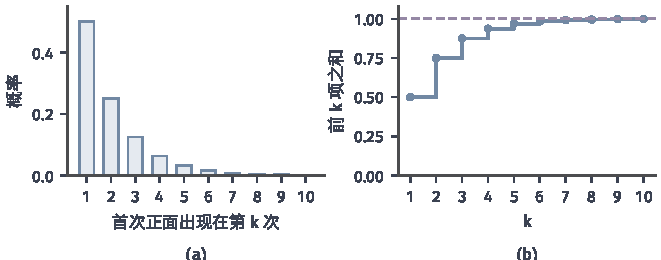
\includegraphics[width=112mm]{figures/07-probability/01-elementary-probability/matplotlib/cprob-first-head/figure.pdf}
  \caption{抛硬币直到第一次正面。(a)第一次正面出现在第$k$次的概率$2^{-k}$；(b)前$k$项之和$1-2^{-k}$，紫色虚线是总和$1$，有限项之和都达不到它。}
  \label{fig:cprob-first-head}
\end{BookInlineFigure}

\paragraph{连续的位置}
在长为$1$的木棍上随机选一个点，点的位置可以是$[0,1]$中的任何实数。所谓“随机”，自然的意思是长度相同的两段被选中的机会相同。问点落在$(0.2,0.5]$中的概率是多少？

计数比在这里给不出答案：$(0.2,0.5]$与$[0,1]$都有无穷多个点，比值是“无穷比无穷”。可以先用有限模型逼近：在$(0,1]$上取$n$个等距位置$k/n$，$k=1,\ldots,n$，让它们等可能。这是一个古典模型，事件“落在$(0.2,0.5]$中”的概率是其中位置的个数除以$n$。

图~\ref{fig:cprob-grid-uniform}(a)显示，随着$n$增大，这个计数比趋于区间的长度$0.3$。例如$n=10$时恰有$3$个位置，比值是$0.3$；$n=7$时有$k=2,3$两个位置，比值是$2/7\approx0.286$。另一方面，图~\ref{fig:cprob-grid-uniform}(b)中单个位置的概率$1/n$趋于$0$。

\begin{BookInlineFigure}
  \centering
  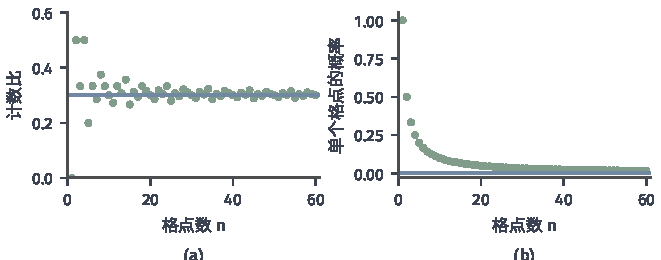
\includegraphics[width=112mm]{figures/07-probability/01-elementary-probability/matplotlib/cprob-grid-uniform/figure.pdf}
  \caption{用$n$个等距位置$k/n$逼近木棍上的随机点。(a)绿点是事件“落在$(0.2,0.5]$中”的计数比，蓝线是区间长度$0.3$；(b)绿点是单个位置的概率$1/n$，趋于蓝线$0$。}
  \label{fig:cprob-grid-uniform}
\end{BookInlineFigure}

这两个极限提示了连续情形的做法：区间的概率由长度给出，不由点数给出；每个单点的概率都是$0$，但每个点都可能被选中。概率为零不等于不可能，这在有限的古典模型中不会发生，那里$\mathbb{P}(A)=0$当且仅当$A=\varnothing$。长度的作用在一般情形中由密度承担，单位长度上的概率可以随位置变化，第~\ref{chap:random-variables}章用积分计算这类概率。

\paragraph{三类情形的统一}
表~\ref{tab:cprob-models}把本节的几种情形放在一起。它们分配概率的方式不同，但都应当满足非负、总量为$1$、互斥事件的概率相加这几条要求；可数个结果和连续位置还要求可加性对可数个互斥事件成立。

\begin{BookInlineTable}
  \centering
  \caption{几类概率模型分配概率的方式}
  \label{tab:cprob-models}
  \begin{tabular}{lll}
    \toprule
    样本空间 & 例子 & 事件的概率 \\
    \midrule
    有限，等可能 & 均匀骰子、摸球 & 计数比$\lvert A\rvert/\lvert\Omega\rvert$ \\
    有限，不等可能 & 点数和、偏心骰子 & 所含结果的概率之和 \\
    可数无穷 & 首次正面的次数 & 所含结果的概率之和（级数） \\
    连续位置 & 木棍上的点 & 长度，一般为密度的积分 \\
    \bottomrule
  \end{tabular}
\end{BookInlineTable}

把这些情形纳入同一个框架，需要回答哪些集合可以作为事件、概率怎样对可数个事件相加，以及长度这样的量能定义在哪些集合上。这些问题在第~\ref{chap:probability-spaces}章用概率测度统一回答。在此之前，第~\ref{chap:random-variables}章先用概率表和密度直接处理有限、可数与连续的情形。

\section{本章小结}
\label{sec:cprob-summary}

本章用一个盒子贯穿始终：$3$个黑球、$2$个白球，摸出两个。把这次抽样从头算一遍，就能把本章的概念串起来，并看清各步依赖的假设。表~\ref{tab:cprob-summary}按顺序列出各步。

\begin{BookInlineTable}
  \centering
  \caption{摸球问题中各步的计算与所用假设}
  \label{tab:cprob-summary}
  \begin{tabular}{lll}
    \toprule
    步骤 & 计算 & 所用假设 \\
    \midrule
    样本空间 & 有序对共$20$个 & 记录先后，细到能表达事件 \\
    等可能 & 每个有序对概率$1/20$ & 搅匀后每个球机会相同 \\
    计数 & $\mathbb{P}(H_1\cap H_2)=6/20$ & 分子分母同一口径 \\
    条件概率 & $\mathbb{P}(H_2\mid H_1)=2/4$ & $\mathbb{P}(H_1)>0$ \\
    乘法规则 & $\tfrac35\cdot\tfrac24=\tfrac{3}{10}$ & 条件随已摸结果改变 \\
    全概率 & $\mathbb{P}(H_2)=\tfrac{6}{20}+\tfrac{6}{20}=\tfrac35$ & $H_1,H_1^{\mathrm{c}}$构成划分 \\
    Bayes & $\mathbb{P}(H_1\mid H_2)=1/2$ & $\mathbb{P}(H_2)>0$ \\
    独立性 & 不放回不独立，放回独立 & 放回时乘积空间等可能 \\
    \bottomrule
  \end{tabular}
\end{BookInlineTable}

\paragraph{样本空间与计数}
概率首先要有一个样本空间：它列出一次试验的全部可能结果，事件是其中的子集，一次试验只产生一个结果，却可以让许多事件同时发生。样本空间由记录方式决定，它必须细到能表达所关心的事件。在有限且等可能的前提下，事件的概率是计数比$\lvert A\rvert/\lvert\Omega\rvert$，它满足非负、归一和互斥可加三条性质，补事件公式、加法公式与联合界都从这三条推出。

等可能是对试验的假设，依据是物理的对称性，不是样本点名称的对称。点数和、颜色记录、无序的可重复组合都合并了不同数量的基本结果，不能直接数类别。计数时分子和分母必须在同一个样本空间中数；放回与不放回改变的是样本空间本身。相对频率可以检验等可能假设是否与试验相符，但本章不用它定义概率。

\paragraph{条件与独立}
条件概率把样本范围缩小到已知发生的事件$B$，在其中按原比例重新归一，要求$\mathbb{P}(B)>0$。由它得到乘法规则，可以沿试验过程逐步计算；按划分分组得到全概率公式，再反推来源得到Bayes公式。先验、条件检出概率和后验分别回答不同的问题，$\mathbb{P}(A\mid B)$与$\mathbb{P}(B\mid A)$不能互换。逐次更新时，前一次的后验成为下一次的先验，但每次乘以似然比都要求给定状态时各次观察互不影响。

独立是交事件概率等于乘积这一数量关系，它与互斥不同，也不由“物理上是否有关”决定。多个事件的相互独立要求所有子组的乘积关系，两两独立或只验证全体之交都不够。重复试验中的独立性来自乘积样本空间上的等可能假设，不放回抽样不满足这一假设。条件之下的独立与不加条件的独立是两回事。

\paragraph{边界与下一步}
古典模型严格而具体，但只适用于有限且等可能的结果。结果不等可能时要逐个指定概率；结果有可数无穷多个时，可加性必须推广到可数个事件；结果取连续位置时，单点的概率为零，区间的概率要由长度或密度给出。下一章把试验的结果记录成数值，引入随机变量，用概率表、分布函数和密度描述它取各种值的概率，这三类情形都在那里得到具体的处理。

